%
% You may wish to use some of the following options of the iitthesis
% package:
%
% fullpageDraft      avoid the margins necessary for proper binding and
%   just view or print a draft.
% beforeExam         makes the personal acknowledgements invisible; use
%   this to print the copies you submit initially to the grad school
%   for sending to the examiners (who shouldn't see these). For the
%   final submission, drop this option.
% noabbrevs          no notation & abbreviations list will be included
%   in the thesis.
%
% Additionally, you must specify the degree for which you're writing
% your thesis (MSc/PhD/MArch etc.)
%
\documentclass[PhD,noabbrevs]{misc/iitthesis}
%\usepackage[english,hebrew]{babel}

% Definitions of info fields for the thesis - subject, advisor,
% faculty, acknowledgements, etc. etc. This file must contain Hebrew
% text, so the question of its character set encoding is significant.
% This templated uses the iso-8859-8-i charset (i.e. single-byte logical 
% Hebrew; it's about the same as the windows-1255 codepage, but not the
% same as UTF-8) - and this works with MikTeX 2.9 and using pdfelatex.
% With your TeX distribution you might need to create files in the
% UTF-8 charset.
\authorEnglish{Ran Bernstein}
\authorHebrew{}

\titleEnglish{Laban Movement Analysis and LDA Distributed Monitoring}
\titleHebrew{}

\disciplineEnglish{Computer Science}
\disciplineHebrew{מדעי המחשב}

\supervisionEnglish{This research was carried out under the supervision of Prof.~Assaf Schuster, in the Faculty of Computer Science.}
\supervisionHebrew{}

\thesisbibfiles{back/general}
\thesisbibstyle{alpha}


% Personal acknowledgements (are only used for the post-exam
% version)
\personalAcknowledgementEnglish{
I would like to thank my advisor, my parents and my girlfriend.
}

\personalAcknowledgementHebrew{
}


% The abstract in Hebrew and in English should have its own file.
%
% Notes:
% - You can split this one, and have separate files for the English
%   and the Hebrew abstract
% - regulations require the English abstract contain between 200 and
%   500 words, and the Hebrew abstract contain between 1,000 and 2,000
%   words (making it something between an abstract and an introduction
%   with an overview of results).
% - Be careful with links in Hebrew text (wrap them in \L{}).

% Just write down your abstract here, no special commands necessary except for the \abstractEnglish{
% before this text is used and a closing } at the end of it

\abstractEnglish{
The first chapter of the thesis deals with Laban Movement Analysis (LMA), which is a method for describing, interpreting and
documenting all varieties of human movement. Analyzing movements using LMA is
advantageous over kinematic description of the movement, as it captures
qualitative aspects in addition to the quantitative aspects of the movement. As
such, it has many applications and its popularity is increasing in recent years
as the preferred method for movement analysis in motor research, theater training,
and the development of interactive gaming animations and robotics. In this study
we aimed to develop an automated method for recognizing 18 different Laban motor
elements (motor characteristics) from markerless 3D movement data captured by the
ubiquitous Kinect camera.  Using machine-learning methods we have succeeded to
obtain a recall rate of 38-94\% (65\% on average) and precision rate of 29-100\%
(59\% on average) for the 18 motor elements that were tested.

\par The second chapter of the thesis deal with systems for mining dynamic data streams should be able to detect changes that affect the accuracy of their model. A distributed setting is one of the main challenges in this kind of change detection. In a distributed setting, model training requires centralizing the data from all nodes (hereafter, synchronization), which is very costly in terms of communication. In order to minimize the communication, a monitoring algorithm should be executed locally at each node,
while preserving the validity of the global model (the model that will be computed if a synchronization will occur). For minimizing this communication, we propose the first communication-efficient algorithm for monitoring a classification model over distributed, dynamic data streams. The classification algorithm that we chose to monitor is Linear Discriminant Analysis (LDA), which is a popular method used for classification and dimensionality reduction in many fields. This choice was made due to the strong theoretical guarantee of correctness that we prove on the monitoring algorithm of this kind of model.
In addition to its theoretical guarantee, we demonstrated how our algorithm and a probabilistic variant of it reduce communication volume by up to two orders of magnitude (compared to synchronization in every round) on three real data sets from different worlds of content. Moreover, our approach monitors the classification model itself as opposed to its misclassifications, which makes it possible to detect the change before the misclassification occurs.

}

% Note that various commands don't work that well in Hebrew. Specifically,
% if you're using hyperref, you'll have trouble with \url, \autoref, \cite
% and friends. iitthesis-extra.sty has a workaround: the \disabledlinksL
% command. See the .sty for details, or:
% http://tex.stackexchange.com/q/32466/5640 for

\abstractHebrew{
}


%
% Just write down your abstract here, no special commands necessary except for the \abbreviationsAndNotation{
% before this text is used and a closing } at the end of it

\abbreviationsAndNotation{

}


% Additional machinery relevant to any thesis
% (it's not part of the document class because it's not absolutely
% necessary and not everyone might like it)

\usepackage{misc/iitthesis-extra}

% Definitions useful for anything you write, which you also
% include in any articles, presentations, HW assignments and other
% documents. May contains macros for notation algebra, logic,
% calculus and other fields, as well as general shorthands and
% LaTeX tricks, and package use commands

% General-purpose definitions and inclusions
% you are using in any document 
% (regardless of its class and style files used),
% e.g. package uses:

\usepackage{xspace}
\usepackage{caption}
\usepackage{subcaption}
\usepackage{pgfplotstable}

\usepackage{algorithm}
\usepackage[noend]{algpseudocode}

\usepackage{multibib}
% and macros/command defintions:

%\newcommand{\complexityclass}[1]{{\bf #1}\xspace}
%\newcommand{\NPTIME}{\complexityclass{NP}}

% For this template, we'll only have one single command,
% necessary for including graphics...
\usepackage{graphicx}% http://ctan.org/pkg/graphicx


% Definitions, settings and tweaks for this thesis specifically

% This file should contain your own definitions specific
% only to this thesis;

% What it contains below is used 
% simply for generating dummy text in the sample 
% content provided with the template (see mainchap1.tex);
% so you can safely delete this when creating your own
% thesis

\usepackage{lipsum}
% ... needs a workaround for babel compatibility, see:
% http://tex.stackexchange.com/q/49214/5640
\makeatletter
\renewcommand\lips@dolipsum{%
  \ifnum\value{lips@count}<\lips@max\relax
    \addtocounter{lips@count}{1}%
    \csname lipsum@\romannumeral\c@lips@count\endcsname
    \lips@dolipsum
  \fi
}
\makeatother

\def\qbfox#1{
\count1=0%
\loop%
   \ifnum\count1<#1%
      \advance\count1 by 1%
      The quick brown fox jumped over the lazy dog. %
      \repeat%
      \relax}



% If you are using WinEdt, and using a publication list on the the
% acknowledgements page, and are having problems getting your document
% to compile with the 'PDFLaTeXify' button, try uncommenting the
% following two lines;
% Also, you will need to PDFLaTeXify at least twice, as WinEdt misses
% an extra run. See also:
% http://tex.stackexchange.com/q/41727/5640




\newcites{pubinfo}{Acknowledgement page references}
\def\iitthesisextramultibibdefs{}

\begin{document}

% Front Matter
% ------------

% The following command will typeset the outer cover page, the
% inner title page, the acknowledgements page, etc. - everything
% up to but not including the introduction
\makefrontmatter

% Main Matter
% ------------
%
% To conform to Technion regulations, the main matter should begin
% with an introduction (including a survey of relevant past work):
%

%

\chapter{Introduction}
\label{chap:intro}

\section{Laban Movement Analysis using Machine Learning}
Recent years there has been a surge of interest in automated analysis of
human motor behavior in the fields of robotics, computer science and animation.
Computerized recognition of movement characteristics has many potential
applications: It could be used for detection of personality traits that are
associated with specific motor tendencies \cite{levy2003use} during, for
example, a job interview, and for early detection and/or for severity assessment
of various illnesses characterized by abnormal motor behavior, such as autism
\cite{dott1995aesthetic} , schizophrenia or Parkinson's disease. Automated
emotion recognition from movement, based on associations between certain
emotions and specific motor behaviors \cite{aristidou2015emotion} is another
important application, which may have a variety of uses such as online feedback
to presenters to help them convey through their body-language the emotional
message they want to communicate (e.g., politicians and public speakers or
dancers and actors in training), or recognition of people's emotions during
interactive games such as those played using the Xbox. Automated analysis of
motor behavior can be used also to assess the progression and improvement of
participants in a variety of training programs that employ virtual reality
environment \cite{aristidou2013motion};  it can be used for motion retrieval
from large motion database \cite{kapadia2013efficient} and for movement indexing
and classification \cite{aristidou2013motion} in the field of animation. Lastly,
machine learning of a person's movement patterns has enormous potential for
future, from security identification, to interactive environments. Most of the
studies dealing with automatic analysis of human movement captured 
movement using complex and expensive 3D motion capture systems. However, in
order to implement the many potential uses mentioned above in our everyday life,
we should be able to do such automated analysis using a small, inexpensive
(affordable) and easy to use 3D camera. One such camera that has been
successfully used in interactive games is the Kinect camera. Thus, in this study
we aimed to develop an automated method for recognizing the motor
characteristics of any human movement captured by a Kinect camera. Once the
movement is captured in 3D, its assessment and analysis can be done in various
ways. In this study we chose to develop the computerized recognition of movement
characteristics based on Laban Movement Analysis (LMA).



\section{Linear Discriminant Analysis}
\label{LDAIntro}
In the second chapter of this thesis, we address the problem of mining data streams when the data 
is \textit{distributed} over a large number of nodes with the same data generation process at every node. However, the streaming data is not stationary; notably, it can change over time. Classic examples of real-life prediction problems that involve this kind of change are user preference prediction and fraud detection. In the former, the choices of the user can change over time; in the latter, the fraudulent transactions change constantly to avoid detection. In both, the change can render the prediction model invalid.
In such a setting --- where the model must be updated to stay valid and communication is costly --- the question is \textit{when} to recompute the model. The naive solution for this problem is recomputing the model periodically. The problem with this solution is that it involves needless work if the model changes infrequently, yet may introduce unacceptable errors between scheduled updates. 
In contrast to periodical computation, we focus on \textit{monitoring} the quality of a given model, and recomputing it only as needed. 
\par We focus on linear binary classifiers, using LDA \cite{fisher1936use} as the learning algorithm. This choice is due the popularity of linear classifiers in real applications and that they serve as a platform for more complex classifiers, such as ensemble model in the work of ~\cite{Deva, eSVM}, neural networks in the work of ~\cite{osadchy2015k}, 
and even deep architectures in the work of \cite{ROSS}. Our method is distinct from the previous work in the following two aspects:

\noindent \textbf{Model-Based Monitoring:} 
Monitoring the model and not the misclassifications has an important benefit: the need for synchronization can be detected before the misclassifications occurs. In contrast to most previous work on monitoring a classifier (that utilizes misclassification rates to draw conclusions about the change in the distribution ~\cite{baena2006early, gama2004learning, nishida2007detecting}), we propose to monitor the change in the \textit{model} itself.

\noindent \textbf{Distributed Setting:} Monitoring a classifier has been actively studied in centralized settings. In contrast to these studies, our is one of the very few works that monitor in a distributed setting. In such setting, data is distributed over a large number of nodes and the model is learned globally after synchronization. While the few existing methods for classifier monitoring in distributed settings rely on heuristics (~\cite{AngGZPH13}), our approach is the only one that provides a provable guarantees of correctness.

\thesisbibfiles{bib}
\thesisbibstyle{alpha}
%
\chapter{Laban Movement Analysis of Movements Recorded by Kinect, Using Machine Learning}
\label{chap:firstchap}

\section{Laban Movement Analysis (LMA)}
LMA is a well-established and widely accepted systematic language for describing
and documenting movement. LMA's comprehensiveness as a motor analysis method
could be inferred from its diverse use in research: it has been used to evaluate
fighting behaviors of rats \cite{foroud2003development}, to analyze behavior of
nonhuman animals in naturalistic settings \cite{fagan1997observing}, to diagnose
autistic individuals \cite{dott1995aesthetic}, to evaluate motor recovery of
stroke patients \cite{foroud2006changes}, and to characterize the development of
infants' reaching movements \cite{foroud2012consummatory}. In recent years it
gained additional popularity among computer science researchers who have used it
in studies that describe, recognize or create bodily emotional expressions for
applications in human-robot interactions, interactive games such as the Xbox,
and in animations \cite{camurri2003recognizing,rett,
Zacharatos, lourens2010communicating, zhao2005acquiring,masuda2009emotion,
masuda2010motion}, and recently it has even been attempted, through the use of
EEG, to identify the brain mechanisms underlying the production of some of the
LMA motor elements \cite{cruz2014neural}. In addition, some studies have found
correlations between some Laban motor elements and personality traits or
emotional states \cite{levy2003use, shafir2015emotion}.
\par Analyzing movements using LMA is advantageous over other methods, as it
captures various qualitative \textbf{motor elements} (movement characteristics)
in addition to quantitative (kinematic) aspects of the movement. LMA categorizes
movement with four main components: Body, Effort, Shape, and Space.
\textbf{Body} (i.e. which \textit{body parts} move) and \textbf{Space} (i.e. the
direction of movement such as Vertical:
\underline{Up/Down}, Sagittal: \underline{Forward/Back} or Horizontal: to the
side), describe how the many spatial-temporal body and limb relationships
change. The category of Body also
includes specific common \textit{body actions} such as jump and walk.
\textbf{Effort} describes the qualitative aspect of movement expressive of a
person's inner attitude
towards movement via four Effort factors: Weight, Time, Space and Flow. Each
Factor identifies movement on a continuum between two poles: fighting against
the motor quality of that factor and indulging in that quality. 
1) \textbf{\textit{Weight Effort}}, identifies the amount of force or pressure
exerted in movement, on the continuum from \underline{Strong} to \underline{Light} (and
movements lacking weight activation, i.e., \underline{Passive/Heavy} movement); 
2) \textbf{\textit{Time Effort}} identifies the degree of urgency or
acceleration/deceleration involved in a movement, i.e., \underline{Sudden} or
\underline{Sustained} movement; 
3) \textbf{\textit{Space Effort}}, describes the focus or
attitude towards a chosen pathway, i.e., is the movement \underline{Direct} or
\underline{Indirect} and 
4)~ \textbf{\textit{Flow Effort}} describes the element of control or
the degree to which a movement is \underline{Bound}, i.e., controlled by muscle
contraction, versus \underline{Free}, i.e., being released/liberated.
Finally, \textbf{Shape} refers to the way the body 'sculpts' itself in space: It
describes the changes in the relationship of body parts to one another and to
the surrounding environment that occur when a body moves (e.g., whether the body
\underline{Encloses} or \underline{Spreads, Rises} or \underline{Sinks}, etc.).
In addition, LMA examines other movement characteristic, such as the
\textbf{phrasing} of the movement, which means the
way movement elements are sequenced into action. Analogous to phrasing in music,
a motor phrase can be \underline{rhythmic} (repetitive), \underline{even}
(monotonous), etc.
(For a more detailed and systematic description of LMA see
\cite{bartenieff1980body,studd, fernandes2014moving}).
\par As can be seen from this short description, LMA is very thorough. It
captures a variety of movement dimensions, and has therefore become the preferred method
for movement analysis used by many scientists. Indeed, in a recent study that
used both Effort-Shape (part of LMA) and kinematic analyses to identify movement
characteristics associated with positive and negative emotions experienced
during walking, more differences among emotions were identified with
Effort-Shape analysis than with kinematic analysis \cite{gross2012effort} , and
both Chi et al.,\cite{chi2000emote} and Masuda et al.,\cite{masuda2010motion}
chose to develop a computer generated animation \cite{chi2000emote} or robotic
\cite{masuda2010motion}  system that transforms simple movements into
emotionally expressive movements, by modifying certain movement parameters of
the animated character or robot, based on LMA. Thus, we have chosen to use LMA
for the purpose of developing the automated method for recognizing movement
characteristics.
\par Because LMA is a comprehensive system with tens of different motor
characteristics, and because many of the current applications for automated
analysis of movement have to do with creation or recognition of emotional
expressions in movements, we  focused this study on identification of the 18
Laban motor elements (Table \ref{mixedSummary} in the results section)
found to be associated with specific emotions[18]. Thus, we created a data base
of movements captured by a Kinect camera and developed machine learning-based,
algorithms for automated identification of the 18 Laban motor elements
expressive of emotion, from our Kinect data.

\section{Method}
\subsection{Kinect Sensor Data}
The Kinect Software Development Kit (SDK) detects the skeleton of the videotaped
moving person and provides the 3D coordinates of 24 joints along this skeleton,
as seen in Fig. ~\ref{skeleton}.

\begin{figure}[h]
\centering
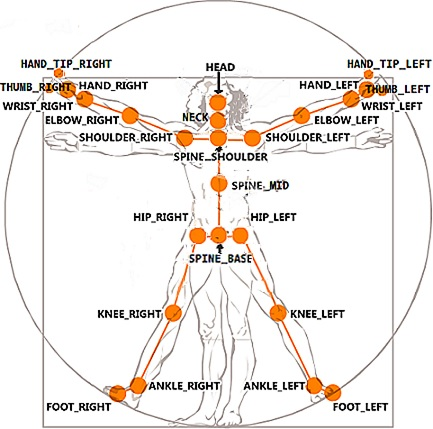
\includegraphics[width=2.5in]{graphics/Laban/skeleton.jpg}
\caption{Skeleton positions relative to the human body}
\label{skeleton}
\end{figure}

The coordinates of these joints are given in a
“real world” coordinate system whose origin [0,0,0] is in the sensor and whose
x, y, and z axis are as depicted in Fig. \ref{Coordinate} below. Data were
collected by the Kinect camera at 30 Hz.


\begin{figure}[h] \centering
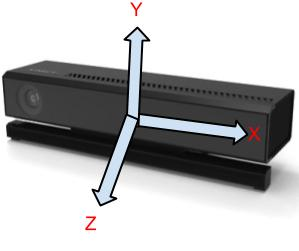
\includegraphics[width=2.5in]{graphics/Laban/KinectV2CoordinateSystem.jpg}
\caption{Kinect Coordinate System}
\label{Coordinate}
\end{figure}

\subsection{Clip collection}
In order to develop the ability to automatically identify Laban motor elements
we had to ensure that the movements in the data set used for the machine
learning, included those elements. Thus, for this study, we generated two
specific data sets:
\begin{itemize}
  \item CMA dataset: This dataset consisted of clips of movements performed by
  Certified (Laban) Movement Analysts experts (CMAs). Six CMAs performed
  movement sequences of approximately 3 seconds long, which consisted of different 
  combinations of LMA motor elements. Before each movement sequence (clip) the
  CMAs were given a list of 2-4 Laban motor elements out of the 18 motor elements that 
  were studied, and were instructed to move any movement that they want, as long 
  as it incorporates those required motor elements. Each of the CMAs moved about 
  80 such different combinations of 2-4 motor elements, for a total of 550 clips. 
  To achieve uniform distribution of the Laban qualities over the dataset, in every 
  movement sequence (clip) each CMA was asked to perform actions that included
  several specific motor elements, and nothing but them.
  \item Non-CMA dataset: This dataset consisted of movement sequences performed
  by two people without a background in LMA, who were asked to move as if they are 
  performing different every-day tasks such as greeting a friend or playing with 
  a balloon. Their movements lasted also about 3 seconds long and a total of 30
  such clips were collected. Their movements were tagged by a CMA who determined 
  which of the 18 Laban qualities that we tested in this study appeared in each of 
  their movement sequences (clips).
\end{itemize}
\par Both the CMAs and non-CMAs performed their movement sequences within a
$316\times 128$ cm rectangular frame marked on the floor, whose front side was
located 272 cm from the front of the Kinect Camera. By limiting the space within which the people could move, we ensured that the Kinect camera could capture all of the mover's joints 
at any point in time throughout the movement sequence, and no joint came out of the 
camera range.
\subsection{Multi Label Classification}
In multi-label learning each instance is associated with multiple labels
simultaneously, and the number of labels is not fixed from instance to instance. 
The task in this learning paradigm is to predict the label set (Laban motor elements 
in our study) for each new unseen instance (skeletal recording, i.e., clip), based on 
analysis of training instances with known label sets. In other words, by providing the 
system with clips identified by the Laban motor elements they include, the system 
learns to recognize the appropriate motor elements in new clips which it didn't
``see'' before. In this study we dealt with three different classification problems, 
with increasing complexity. 
First we provided the system with clips and the Laban motor elements included 
in them from one CMA, and taught it to recognize those Laban elements in new unseen clips 
of the same CMA. This method can be developed to teach a system to recognize qualities 
in an individual's unique movement expression. In the second step we taught the
system to recognize the Laban elements in the clips (i.e., movements) of each new CMA 
based on the labeled clips of the other CMAs. Lastly, based on all CMAs dataset, the system 
learned to recognize those motor elements in clips of the non-CMAs' movements. 
\subsubsection{Clip Labeling}
Clips were labeled by the motor elements in the instructions for each clip, with
the assumption that as experts in LMA, the CMAs indeed performed the required elements. 
Thus, the instructions given to the CMAs regarding which motor elements to move, 
were used as the ground truth for labeling the motor elements in each clip of the CMA data set. 
Labeling of the motor elements in the movements of the non-CMAs was done by one of the authors 
who is a CMA who observed those movements.
\subsection{Feature Extraction}
The machine learned to recognize the different Laban qualities by extracting
many features from each movement, and by learning from the training-set clips
which features characterize each motor element. It then identified the Laban
elements in new clips based on the features extracted from the movement in those
new clips.
\par To enable the CMAs to express the motor elements in a variety of different
movement sequences, we did not want to constrain the lengths of the clips to be
exactly 3 seconds. Thus, in order to get feature vectors of uniform length
(regardless of the original length of the clips), every extracted feature was a
function of the whole clip, i.e., all the extracted features were in whole clip
granularity.
\par Two groups of features were extracted: the first was relatively small,
containing a handful of features, each of which was designed to portray a
specific Laban motor element based on “translation” of the meaning of that
element into kinematic terms. The second group contained about 6000 features,
and exploited the rich data that was provided by the Kinect software, by
extracting from every joint in the skeleton, its derivatives: angular velocity,
acceleration and jerk. For every time series of [joint $\times$ dimension $(X,
Y, Z) \times$ derivative], we calculated about 20 statistics, such as: mean, variance,
skewness, kurtosis.
\par The following are examples for some of the manually composed features that
were designed to portray some of the specific motor elements, and for each of which
we also calculated the 20 statistics:
\subsubsection{Advance and Retreat}
Advance and retreat are two Laban motor elements that incorporate changes in the
Shape of the body in the sagittal plane, where part of the body's core (axial
skeleton), usually the upper body, moves forward (Advance) or backward (Retreat)
in relation to the lower part of the body. These elements were quantified by
projecting the velocity vector of the Center of Mass (CM) on the vector of the
front of the body. The CM was approximated in this case by the average of all
the joints. The front of the body was approximated by the perpendicular vector
to the vector between the Left Shoulder (LS) and the Right Shoulder (RS). From
the definition of CM of a physical system we calculate:
\begin{equation}
\vec{P}_{CM}(t) = \sum_{j \in Joints} \alpha_{j}\vec{P}_{j}(t),
\end{equation}
\begin{equation}
\vec{P}_{shoulders}(t)=\vec{P}_{LS}(t)-\vec{P}_{RS}(t),
\end{equation}
the front is perpendicular to $\vec{P}_{shoulders}$, so we can easily calculate it with:
\[\vec{P}_{front}=\vec{P}_{shoulders}\left( \begin{array}{ccc}
0 & 0 & 1 \\
0 & 1 & 0 \\
-1 & 0 & 0 \end{array} \right),\]
\begin{equation}
S_{sag}(t) = \vec{P}_{CM}(t)\cdot\vec{P}_{front}(t),
\end{equation}
\begin{equation}
\vec{F}_{sag} = \phi([S_{sag}(1), \ldots S_{sag}(n)]),
\end{equation}
where $\vec{Pj(t)}$  is the vector of the position of joint $j$ (as we get it
from the Kinect) in time $t$ in a clip with n frames, and $\alpha_{j}$ is a
coefficient proportional to the mass around the joint. $\phi$ is the function
that creates the 20 statistics from the time series.
$S(t)$ is a scalar in the time series at time $t$.  $F$ denotes the calculated
features for Advance and Retreat, and $sag$ stands for sagittal.
\subsubsection{Spread and Enclose}
These are two Laban motor elements describing opposite changes in the Shape of
the body in the horizontal plane. In Spread the body becomes wider and when
Enclosing, the body becomes narrower. These elements were quantified by
measuring the changes in the average distance between every joint and the
vertical axis of the body that extends from the Head $(H)$ to the Spine Base
$(SB)$:
\begin{equation}
d_{j} = \frac{\left|(\vec{P}_{j}-\vec{P}_{SB})\times
(\vec{P}_{j}-\vec{P}_{H})\right|}{\left|\vec{P}_{H}-\vec{P}_{SB}\right|},
\end{equation}

\begin{equation}
S_{horiz}(t) = \sum_{j \in Joints} d_{j}(t),
\end{equation}

\begin{equation}
\vec{F}_{horiz} = \phi([S_{horiz}(1), \ldots S_{horiz}(n)]),
\end{equation}
Where $P, S, \phi, CM$ and $F$ are defined as in the previous paragraph, and
$horiz$ stands for horizontal.
\subsubsection{Rise and Sink}
Rise and Sink are changes in the Shape of the body in the vertical plane, where
during Rising, the body elongates upward and during Sinking the body goes down
and shortens. The distinction between these two Laban motor elements was
quantified by measuring the average distance on the $Y$ axis of each joint from
the $CM$:
\begin{equation}
S_{vert}(t) = \sum_{j \in Joints}
\left|\vec{P}_{j}-\vec{P}_{CM}\right|,
\end{equation}
\begin{equation}
\vec{F}_{vert} = \phi([S_{vert}(1), \ldots S_{vert}(n)]),
\end{equation}
where $P, S, Ø, CM$ and $F$ are defined as previously and $vert$ stands for
vertical.
\subsubsection{Sudden and Sustain}
Sudden and Sustain are two opposing motor elements of the Time dimension of the
Effort factor of the movement.  The distinction between them was quantified by
calculating the skewness of the acceleration, based on the assumption that the
acceleration of a sudden movement has higher values at the beginning of the
movement, i.e. is skewed to the left.
\begin{equation}
\vec{V}_{j}(t) = \vec{P}_{j}(t+1) - \vec{P}_{j}(t),
\end{equation}
\begin{equation}
\vec{a}_j(t) = \vec{V}_{j}(t+1) - \vec{V}_{j}(t),
\end{equation}
\begin{equation}
Skew_j = \frac{1}{n}\sum_{i=1}^{n}(\frac{a_j(t) - \mu}{\sigma})^3
\end{equation}
Where $\vec{Pj(t)}$ is the vector of the position of joint $j$ in time $t,
\vec{Vj(t)}$ is the vector of the velocity of joint $j$  in time $t$, $\mu$ and
$\sigma$ are the mean and standard deviation of the accelerations ($aj(t)$), and
$n$ is the length of the time series (clip). 
\subsection{Performance Evaluation}
From a statistical point of view, for every clip we had 18 possible labels
(Laban motor elements). The movement in each clip was constructed from a
combination of 2-4 of these elements, which meant that there was about 85\%
chance that a certain element will not appear in a clip. Due to this sparsity,
accuracy (defined as the percentage of clips that have been labeled correctly
out of the total number of clips) alone was not a relevant metric for
performance evaluation, since one could get 85\% accuracy by stating that for
every clip none of the motor elements appear in it. However, if we define Truly
Positive Clips (TPC) as clips in which the relevant Laban element truly
appeared, and if we define Classified Positively Clips (CPC) as clips that our
classifier found to include the relevant motor element, then we can get a better
performance evaluation by combining precision (defined as the percentage of
retrieved clips that were relevant) and recall (defined as the percentage of
relevant instances that were retrieved) to create the more concise performance
evaluation measure $F1$ score, which was defined as follow:
\begin{equation}
precision = \frac{|\{TPC\}\cap\{CPC\}|}{|\{CPC\}|}.
\end{equation}
\begin{equation}
recall = \frac{|\{TPC\}\cap\{CPC\}|}{|\{TPC\}|}.
\end{equation}
\begin{equation}
F_{1} = \frac{2\cdot precision\cdot recall}{precision+recall}.
\end{equation}
\subsection{Single Task Learning (STL)}
In the single task learning, for each CMA, the machine learned to evaluate for
each Laban motor element separately whether it existed in a certain movement
sequence, based on the features that were detected in that movement sequence
(clip). This was done by a binary decision for every Laban element whether it
existed in that movement sequence or not.
\subsubsection{Feature selection}

For the purpose of the single task learning (STL) from each clip we extracted a
vector of 6120 features, most of which were noisy and redundant and required
massive feature selection in order to conduct the machine learning task. The
feature selection was done in three stages. 
\par In the first stage we computed
p-value for every feature. As seen in Fig. \ref{selection}, filtering out most
of the features yielded better results than not filtering them, where using the
top 10\% of the features was optimal.
\begin{figure}[ht!]
\centering
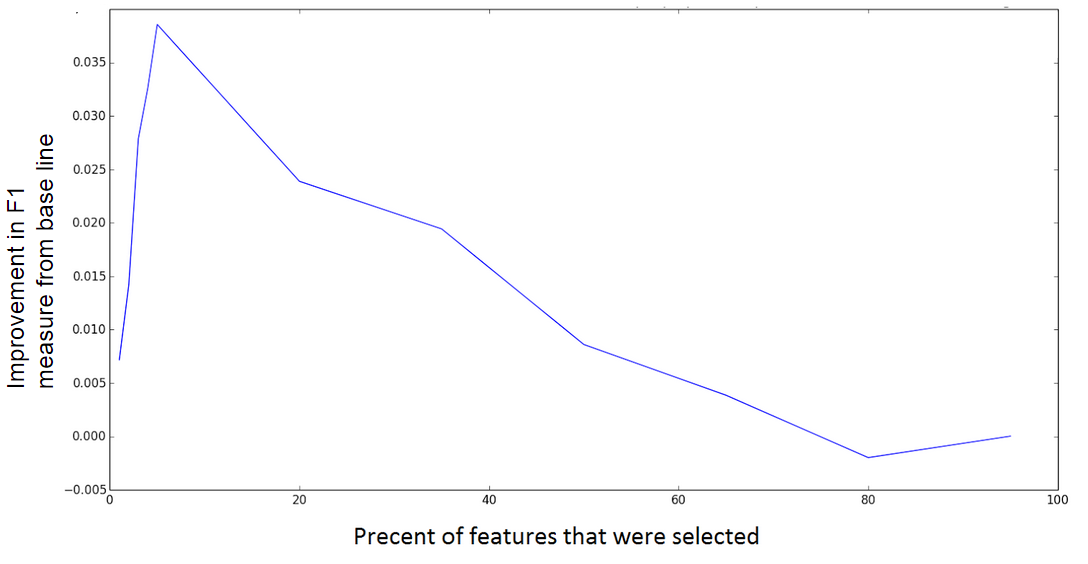
\includegraphics[width=2.5in]{graphics/Laban/featureSelection.png}
\caption{ Influence of the number of features on the performance. The
selection was made according to statistical significance: The blue line is the
difference between the score with and without feature selection. It can be seen
that the optimal percentage of features to select is 10\%}
\label{selection}
\end{figure}
\par The second stage of feature selection was conducted on the features which
were not filtered out in the first stage. In this stage the features were ranked
according to their information gain (IG), which is defined as:
\begin{equation}
       IG(T,f) = H(T) - H(T|f),
\end{equation}
where $T$ is the training set, $f$ is a feature, and $H()$ is the information
entropy of a dataset. During this stage 60\% of the features were selected. 
\par For the third stage of feature selection, which was performed on the
features surviving the first and second stage, we conducted a Least Absolute Shrinkage
and Selection Operator (LASSO) regularization \cite{lasso}. At the end of this
three stages process, for each motor element different number of features were
selected, which were 5-20\% of the original number of features.

\subsection{Multi- Task Learning}
Multi Task Learning (MTL) framework \cite{caruana1997multitask} is an approach
to multi-label learning that learns each task (i.e., each problem solving)
simultaneously with other
tasks (with solving other related problems), using shared representations, even
when the tasks are different. In our study MTL was achieved by simultaneously
learning to recognize all 18 Laban motor elements. Unlike STL, which trains a
separate model for every task (i.e., in our study, for learning to detect each
Laban motor element separately), and in which the data might be represented for
each learning task differently, the goal in MTL was to improve the performance
of learning algorithms by learning classifiers for multiple tasks jointly. MTL
works particularly well when all the tasks have some commonality and are
generally slightly under sampled. For the MTL we used Multitask Elastic Net
(MEN) regularization, which is the multi-task regularization method used by Zou
et al.,\cite{Zou}. MEN promotes sparsity and behaves also as feature selection
mechanism. In MEN the optimization objective is to minimize the following
expression, where $Y$ represents the labels, $X$ represents the samples, and $W$
is the matrix that we want to learn:

\begin{equation}\label{eq:MEN}
\|Y - XW\|^2_F+\lambda_1\cdot\|W\|_{2,1}+\lambda_2\cdot\|W\|^2_F,
\end{equation}

\noindent $\lambda_1$, and $\lambda_2$ are hyper-parameters, where,
\begin{equation}
\|W\|_{2,1} = \sum_i \sqrt{\sum_j w_{ij}^2},
\end{equation}
i.e., the sum of norm of each row (also known as mixed norm), and
\begin{equation}
\|W\|^2_F = \sum_i{\sum_j w_{ij}^2},
\end{equation}
\par Feature selection for the MTL was carried out by averaging the statistical
significance of each feature with respect to all of the tasks. This was in
contrast to the single task learning, where every task had its own feature
selection.

\section{Results}
\subsection{Single-Task Learning}
\begin{figure*}
	\centering
	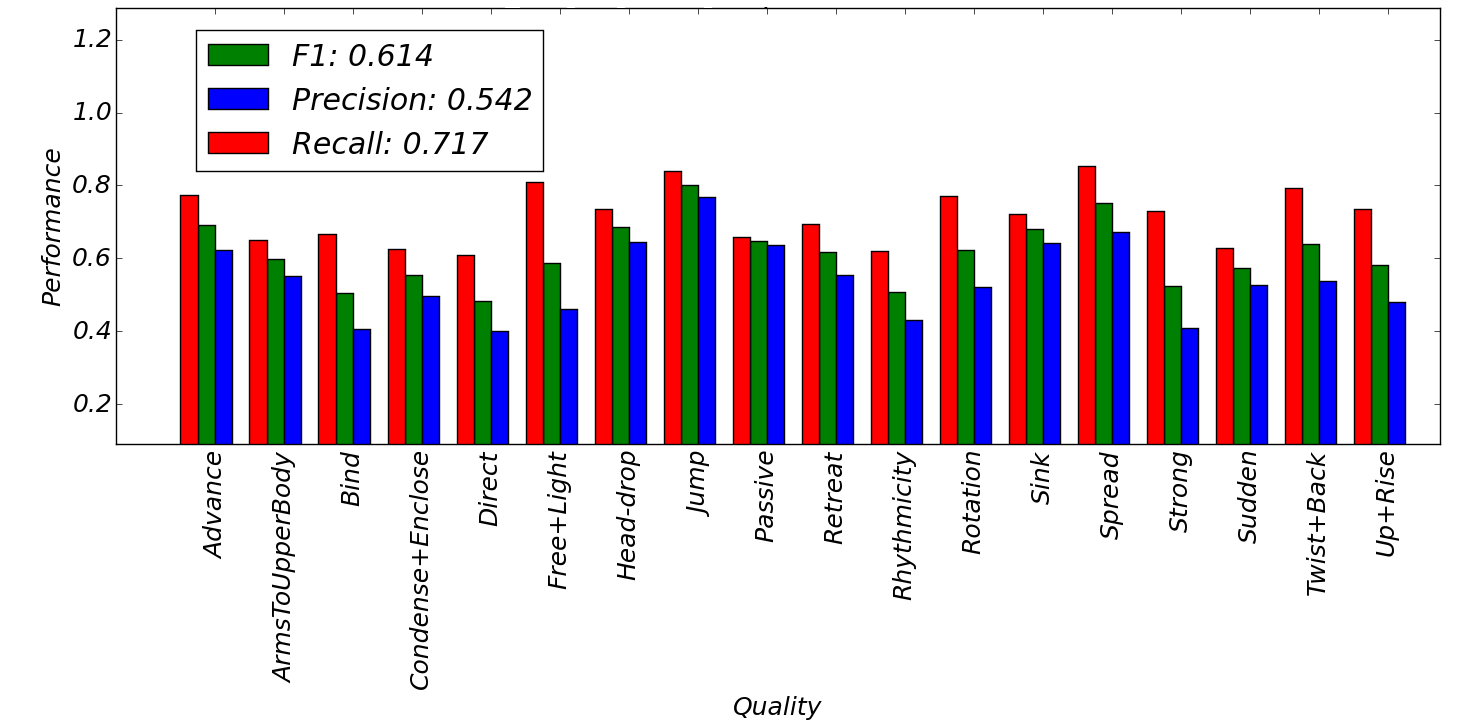
\includegraphics[width=\textwidth, height=70mm]{graphics/Laban/oneCMAFinalWithoutTitle.png}
	\caption{Recall, precision and F1 score of each Laban quality separately. The
	evaluation was conducted on a dataset that was captured on only one CMA.}
	\label{oneCMAFinal}
\end{figure*}
In the STL we used as training set 80\% of the clips produced by each CMA to
 teach the machine to recognize each motor element in the other 20\% of the
 clips performed by the same person. Fig. 4 demonstrates the precision, recall
 and F1 for each of the Laban qualities for the first CMA whose data was
 collected. As can be seen in Figure 4, the performance varied from one Laban
 motor element to another and was about 40-85\% for precision and recall. F1
 values were in between the values for precision and recall, and on average for
 all Laban elements were 0.6.
\subsection{Multi-Task Learning}
\subsubsection{Evaluation performance of each Laban quality}
The MEN regularization was performed on all the clips of all 6 CMAs that
participated in the study.  As a result, 282 features were selected (same
features for all of the tasks). The performance of every motor element as
classified by the MEN regularization is presented in Table \ref{mixedSummary}.
\begin{table}[!h]

%% increase table row spacing, adjust to taste
%\renewcommand{\arraystretch}{1.3}
% if using array.sty, it might be a good idea to tweak the value of
%\extrarowheight 
%as needed to properly center the text within the cells

\caption{Precision, recall, and F1 score of each Laban motor element that resulted from the MTL performed on all clips from all CMAs. The F1 average and standard deviation over the motor elements are shown in the last row of the table}
\label{mixedSummary}
\centering
\begin{tabular}{|p{3cm}|p{0.9cm}|p{0.9cm}|p{0.9cm}|}
\hline
Motor Element&Precis-ion&Recall&F1 score\\\hline
Jump&0.89&0.81&0.85\\\hline
Twist and Back&0.69&0.85&0.76\\\hline
Sink&0.62&0.79&0.69\\\hline
Rhythmicity&0.59&0.72&0.65\\\hline
Spread&0.55&0.76&0.64\\\hline
Head drop&0.60&0.66&0.63\\\hline
Rotation&0.66&0.60&0.63\\\hline
Free and Light&0.45&0.94&0.61\\\hline
Up and Rise&0.67&0.54&0.60\\\hline
Condense and Enclose&0.44&0.84&0.58\\\hline
Arms To Upper Body&0.67&0.54&0.60\\\hline
Advance&1.00&0.38&0.55\\\hline
Retreat&0.50&0.59&0.54\\\hline
Passive&0.40&0.85&0.54\\\hline
Bind&0.44&0.61&0.51\\\hline
Direct&0.56&0.49&0.52\\\hline
Sudden&0.61&0.41&0.49\\\hline
Strong&0.29&0.42&0.34\\\hline
\textbf{Average}&\textbf{0.59}&\textbf{0.65}&\textbf{0.60}\\\hline
\textbf{SD}&\textbf{0.17}&\textbf{0.17}&\textbf{0.11}\\\hline
\end{tabular}

\end{table}
\subsubsection{Multi-task vs. Single-task learning}
The generalization ability of the model was enhanced, compared to that in the
STL, by the fact that the decision of which features to select was influenced by
all the motor elements. The most significant improvements were in the Laban
elements that performed worse in the single task learning setting (Strong and
Sudden for example). As seen in Table \ref{MultitaskVsSeparated}, the multitask
learning improved the overall F1 score  by 4\% compared to the STL.
\begin{table}[ht]
\caption{Multitask vs Single task learning performance evaluation on a data set of several CMA's.}
   \label{MultitaskVsSeparated}
  	\centering
	\begin{tabular}{|p{1.8cm}|p{1.8cm}|p{1.8cm}|}
	\hline
	Metric&Single task&Multitask\\\hline
	Precision&0.46&\textbf{0.59}\\\hline
	Recall&\textbf{0.71}&0.65\\\hline
	F1&0.56&\textbf{0.6}\\\hline
	\end{tabular}
	
\end{table}

\begin{figure}
\centering
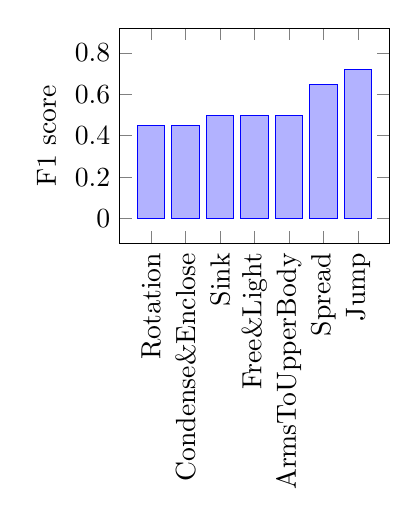
\begin{tikzpicture}
\begin{axis}[
    ymin=0,
    ymax=0.8,
    width=5cm,
    ybar stacked,
    enlargelimits=0.15,
    ylabel={F1 score},
    symbolic x coords={Rotation,Condense\&Enclose,Sink,Free\&Light,ArmsToUpperBody,Spread,Jump},
    xtick=data,
    x tick label style={rotate=90,anchor=east},
    ]
\addplot+[ybar] plot coordinates  {(Rotation,0.45) (Condense\&Enclose,0.45) (Sink,0.5) 
		(Free\&Light,0.5) (ArmsToUpperBody,0.5) (Spread, 0.65) (Jump,0.72)};

\end{axis}
\end{tikzpicture}
\caption{Performance on ordinary  people (non-CMAs) instructed to perform several tasks.}
\label{nonCMAs}
\end{figure}

\subsubsection{Evaluation performance for movements of unseen CMA}
In this experiment the test set was taken from the clips of one CMA while the
training set was composed from the clips of all other 5 CMAs. Testing was
performed for each CMA separately and the results were averaged over all six
CMAs. Performance as measured by F1 degraded on the unseen CMA from 0.6 to 0.57.
This degradation seems mild considering the large variation/diversity among
clips from one CMA to another, as every CMA performed different gestures, in
different postures (some sitting and some standing) and in different contexts
(some were dancing while some were acting).
\subsubsection{Evaluation performance for everyday movements of non-CMAs}
The data set of non-CMAs consisted of several daily movements two people were
asked to do, such as pretending to greet a friend or play with a balloon. This
data set was small, and the people were instructed to do movements that we hoped
would include the Laban motor elements that we have examined in this study, but
we had no direct control over the exact movement they chose to do or the motor
elements included in those movements. A CMA who watched those movements
determined which of the 18 Laban motor elements examined in this study appeared
in those movement sequences. As shown in Fig 5, which describes the learning
performance for this data set, it turned out that only 7 motor elements of the
18 examined in this study appeared in those people's movements. Performance as
measured by average F1 degraded from 0.57 for an unseen CMA to 0.54 for a
non-CMA.


\thesisbibfiles{bib}
\thesisbibstyle{alpha}
\chapter{LDA Model Monitoring in Distributed Systems}
\label{chap:secondchap}

\section{Related Work}
Monitoring dynamic data streams is a broad topic that has been addressed in different research communities. Within this field, we focus on detecting a change in the data stream that renders the prediction model invalid. 
In distributed settings, this problem is even harder and referred to as \textit{distributed monitoring}, and it is concerned with designing local tests for monitoring a function that is defined globally over all the nodes in the system.
Our approach to this problem is to define a constraint over the local data (at each node) that guarantees the validity of the global model. If local data (in one or more nodes) does not meet the local condition, it leads to synchronization. The synchronization process has large communication costs, and the goal of the distributed monitoring methods is thus to minimize the number of synchronizations. Most of the work on distributed monitoring has been concerned with simple functions of the data, such as linear functions in the work of ~\cite{keralapura2006communication} and ~\cite{kashyap2008efficient} or monotonic functions in the work of \cite{michel2005klee}.
For non-linear functions, examples include work on monitoring the value
of a single-variable polynomial as in the work of ~\cite{shah2008handling},
and eigenvalue perturbation as in the work of ~\cite{huang2007communication}.
While the previous work handled specific families of functions, we chose to use \textit{geometric} approach for monitoring \textit{arbitrary} functions over distributed streams, as was proposed, later extended and generalized in \cite{sharfman2007geometric, keren2014geometric, keren2012shape}. A recently introduced work by ~\cite{gabel2015monitoring} on monitoring Least Square Regression (LSR) using geometric monitoring is the closest to ours, but our problem is more complex: unlike the global scatter matrix (required by LSR) the global covariance matrix (required in LDA) is not the mean of the local covariance matrices which makes the monitoring problem more much harder.

\section{Problem Definition}
We first describe the Linear Discriminant Analysis (LDA) algorithm and then define the monitoring problem. 

\subsection{Linear Discriminant Analysis}%\\ \par
LDA seeks a linear combination of features that characterize or separate two or more classes of samples.
The resulting combination may be used as a linear classifier, or for dimensionality reduction before later classification.

In LDA the problem is approached by assuming that the conditional probability
density functions $Pr(\vec x|y=p)$ and $Pr(\vec x|y=q)$ are both normally distributed with
mean and covariance parameters $(p, B_p)$ and
$(q, B_q)$, for two target classes $P$ and $Q$ respectively.
${(x_1,y_1),\ldots,(x_n,y_n)}$ are i.i.d. samples, $x_i \in \mathbb{R}^d$
and $y_i \in \{0,1\}$.

We seek a linear transformation (model), $w \in \mathbb{R}^d $,
that maximizes the separation between the classes, where the separation is
defined to be the ratio of the variance between the classes to the variance
within the classes:
\begin{equation}
S := \frac{\sigma^2_{between}}{\sigma^2_{within}} = \frac{(w^T (p -
q))^2}{w^T(B_p+B_q)w}.
\end{equation}
Solving the maximization problem yields that the decision criterion is a threshold on the
dot product
\begin{equation*} \label{eq:decision}
w \cdot x > c
\end{equation*}
where
\begin{equation} \label{eq:w}
w \propto (B_p+B_q)^{-1}(p - q)
\end{equation}
\begin{equation} \label{eq:c}
c = \frac{1}{2}(T-{p}^T S_p^{-1} {p}+{q}^T S_q^{-1} {q}).
\end{equation}
In this work we monitor $w$, and will refer it as the classification \textit{model}.

\subsection{Monitoring Problem}
We denote $k$ as the number of nodes and $W$ as the number of samples in a node.
Our model uses discrete time (hereafter, rounds). Every node receives a new sample
in a round. We use the \textit{sliding window} model, every node keeps two sliding windows (one for each class) of length of $W/2$. As a node receives a new observation, it replaces the oldest one from its class.
$x^i_j$ and $y^i_j$ are the $j$'th sample and label in the $i$'th node
and $x_{old}^i(p)$ and $x_{old}^i(q)$ are the oldest samples from each class in
the sliding window of the $i$'th node.
As data evolves, it is possible that the previously computed model
no longer matches the current true model. Let $w_0$ be the existing model (vector of weights of a linear classifier), previously computed at some point in the past (the synchronization time), and let $w$ be the \textit{true} LDA model (the hypothetical model that synchronization would yield if it occur).
We wish to maintain an accurate estimation $w_0$ of the current global LDA model, $w$.
For the classification purpose, the most important property of a linear classifier is its direction. Therefore, we monitor the change in this direction: given a threshold $T$, our goal is to raise an alert if
\begin{equation} \label{eq:coneCritiria}
\frac{<w,w_0>}{\parallel w \parallel \parallel w_0 \parallel}  < T.
\end{equation}
i.e. if the angle between $w0$ and $w$ is above a certain threshold (inner product between unit vector is the $cosine$ of the angle between them).

%Due to the complexity of Eq. \ref{eq:coneCritiria},
%we will monitor a simpler problem whose solution also satisfies
Due to the complexity of condition \ref{eq:coneCritiria}, we will monitor a restriction of it: we replaced the cone containment condition to a  sphere containment condition, i.e., 
%Eq. \ref{eq:coneCritiria}: the maximal volume sphere of which $w_0$ is its center
%that resides completely inside the cone from Eq. ~\ref{eq:coneCritiria}.
%This sphere is defined by
\begin{equation} \label{eq:critiria}
||w-w_0||   >  R_0,
\end{equation}
where $R_0 := ||w_0|| \sqrt{1-T^2}$ is the radius of the maximal volume sphere of which $w_0$ is its center and resides inside the cone from condition \ref{eq:coneCritiria}.
%In other words, we replaced containment by distance from the boundary.
%Empirical evaluation showed that the values of
%$1-\frac{<w,w_0>}{||w||||w_0||}$ and $||w-w_0||$ are
%highly  correlated, thus in practice, Eq. \ref{eq:coneCritiria}
%can be replaced by Eq.\ref{eq:critiria}.


\section{Monitoring Distributed LDA With Convex Subsets}
Monitoring distributed LDA models is difficult because the global model cannot be inferred from the local model at each node. Even when all current local models $w_i$ are similar to the precomputed local models $w_0$, the current global model $w$ may be very different from the precomputed model $w_0$: consider the example in Figure \ref{NegativeExample} with $k = 2$ nodes and dimension $d =2$. The angle deviation of the global model (shown in solid lines) is large (45 degrees) even though the local models (shown in dashed lines) are identical to what they were at the initial point.

\begin{figure}[h]
\centering
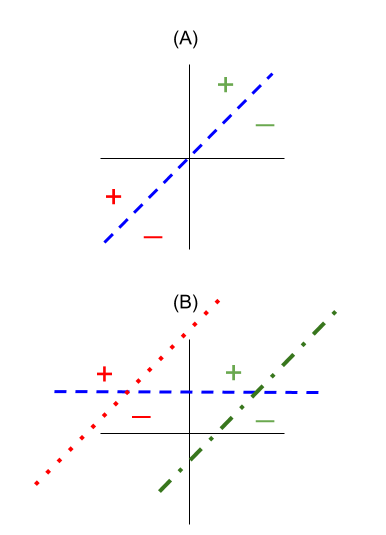
\includegraphics[width=60mm, height=9cm]{graphics/LDA/NegativeExample.png}
\caption{Example of incorrect monitoring by applying LDA locally. The
initial state of the data is presented in (A) and the state at a later point
is shown in (B). In (B) every node (green and red dashed lines) calculates the same angle
for the separator as it was in (A). But it can be
seen that the global separator's (blue solid line) angle has changed
significantly.}
\label{NegativeExample}
\end{figure}


\par To overcome this difficulty, we impose constraints on local data at the nodes, rather than on the function of the global aggregate. Given a function of the average of all local data and the threshold, we compute a ``good'' convex subsets, called \textit{safe zones}, for each node.

\par As we show below, convexity plays a key role in the correctness of this scheme. As long as local data stay inside the safe zones, we guarantee that the function of the global average ---  the euclidean distance between the true global model to the one that was computed in the last synchronization (hereafter, model drift) --- does not cross a threshold.
Nodes communicate only when local data leaves the
safe zone, which we call a safe zone \textit{violation} (hereafter,
violation). Once that happens, violations can be resolved,
for example by synchronization.
In other words, we want to impose conditions on the local
data at each node so that as long as they hold, $||w-w_0||<R_0$, i.e., the global model is valid.

\subsection{Notation}
\noindent
We recall that $P$ and $Q$ are the classes in the binary classification problem.
 $(p,q)$ and $(p^i,q^i)$  are the global and local means of classes $P$ and $Q$.
\\$S$ and $S^i$  are the global and local normalized scatter matrices of the feature space:
\begin{equation*}
S^i := \frac{1}{W}\sum_{j=1}^{W}x^i_j(x^i_j)^T
\end{equation*}
\begin{equation*}
S := \frac{1}{Wk}
\sum_{i=1}^k\sum_{j=1}^Wx^i_j(x^i_j)^T=\frac{1}{k}\sum_{i=1}^kS^i.
\end{equation*}
\\Similarly, $u$ and $u^i$ are the distance between the means of the classes, i.e., $u:=p - q$ and $u^i:=p^i - q^i$.
\\ $B$ is the global covariance matrix, which is the sum of the covariance matrices of the two classes, i.e., $B:=B_p+Bq$.
It can be shown that $B=S - pp^T - qq^T$.
%\\B^i:=S^i - p^i(p^i)^T - q^i(q^i)^T$
\\Let $w$ be our current true model. Then, following Eq.~\ref{eq:w}, we can express:
%\\$w(S,\mu_p,\mu_q) := (S - \mu_p\mu_p^T - \mu_q\mu_q^T)^{-1}(\mu_p - \mu_q)$
\begin{equation}
w:=(S - pp^T - qq^T)^{-1}(p-q)=B^{-1}u.
\end{equation}
%In the following the subscript $0$ will denote the state at the time
%of last synchronization.
Let $w_0$ be the existing model, previously computed from $(S_0, p_0, q_0)$
or from $(B_0,u_0)$ at the time of synchronization.
Then,
\begin{equation}
w_0:=(S_0 - p_0p_0^T - q_0q_0^T)^{-1}(p_0-q_0)=B_0^{-1}u_0.
\end{equation}

If $S_0^i$, $p_0^i$ and $q_0^i$ are the local normalized scatter and averages
of the samples in a node at the time of last synchronization, we define the \textit{local drifts} to be:
\begin{alignat*}{1}
& \Delta_s^i:= S^i - S_0^i
\\ & \delta_p^i:= p^i - p_0^i
\\ & \delta_q^i:= q^i - q_0^i.
\end{alignat*}
We define $\Delta_s, \delta_p$, and $\delta_q$ --- the \textit{global drift} vectors of $S, p$, and $q$ --- to be:
\begin{alignat*}{1}
& \Delta_s:= S - S_0 \\
& \delta_p:= p - p_0 \\
& \delta_q := q - q_0.
\end{alignat*}

\begin{remark} \label{average}
It is easy to see that every global drift vector is the average of the local drift vectors:
\begin{alignat*}{1}
& \Delta_s = \frac{1}{k} \sum \Delta_s^i, \\
& \delta_p = \frac{1}{k} \sum \delta_p^i, \\
& \delta_q = \frac{1}{k} \sum \delta_q^i.
\end{alignat*}

\end{remark}

\subsection{Convex Safe Zones}
Each node monitors its own drift vector: as long as current values
at local nodes $(S^i,p^i,q^i)$ are sufficiently similar to their values
at synchronization time $(S^i_0,p^i_0,q^i_0)$, $w_0$ is guaranteed to be close to $w$.
Formally, we define a convex set $\mathcal{C}$ such that:
\begin{equation} \label{convex}
(\Delta_s, \delta_p, \delta_q) \in \mathcal{C} \Rightarrow \parallel w-w_0
\parallel \ < R_0.
\end{equation}
\begin{lemma} \label{averages}
Let $\mathcal{C}$ be a convex set that satisfies Eq. \ref{convex}.
If $(\Delta_s^i, \delta_p^i, \delta_q^i) \in \mathcal{C}$ for all i, then
\begin{equation*}
||w-w_0|| < R_0.
\end{equation*}
\end{lemma}
\begin{proof}
We express $S, p$ and $q$ as their values at synchronization with the addition of the average of the local drift vectors:
\begin{equation}
\begin{split}
\\(S,p,q) & = \frac{1}{k} \sum_i (S^i,p^i,q^j) \\
 & = (S_0,p_0,q_0) + \frac{1}{k} \sum_i (\Delta_s^i,\delta^i_p,\delta_q^i). \\
\end{split}
\end{equation}
From $\mathcal{C}$'s convexity and using Remark \ref{average} we get:
\begin{equation}
\begin{split}
\forall i (\Delta_s^i,\delta^i_p,\delta_q^i) \in \mathcal{C} & \Rightarrow
\frac{1}{k} \sum_i (\Delta_s^i,\delta^i_p,\delta_q^i) \in \mathcal{C} \\
& \Rightarrow (\Delta_s,\delta_p,\delta_q) \in \mathcal{C}.
\end{split}
\end{equation}
Finally, from the definition of $\mathcal{C}$ we obtain:
\begin{equation}
(\Delta_s,\delta_p,\delta_q) \in \mathcal{C} \Rightarrow \parallel w-w_0
\parallel \ < R_0,
\end{equation}
\end{proof}

\subsection{Convex Bound for Local Condition}
We denote the change in the global covariance matrix
\begin{alignat*}{2}
\Delta & := && B-B_0 \\
& = && (S_0+\Delta_S - (p_0+\delta_p)(p_0+\delta_p)^T \\
& && - (q_0+\delta_q)(q_0+\delta_q)^T) \\
& && - (S_0 - p_0p_0^T - q_0q_0^T) \\
& = && - \delta_p\delta_p^T - \delta_q\delta_q^T \\
& && + \Delta_S - p_0\delta_p^T \\
& && - \delta_pp_0^T - q_0\delta_q^T - \delta_qq_0^T.
\end{alignat*}
We break $\Delta$ into its quadratic part,
\begin{equation*}
M:= - \delta_p\delta_p^T - \delta_q\delta_q^T
\end{equation*}
\begin{equation*}
M^i:= - \delta_p^i(\delta_p^i)^T - \delta_q^i(\delta_q^i)^T
\end{equation*}
and its linear part,
\begin{equation*}
L:= \Delta_S - p_0\delta_p^T - \delta_pp_0^T - q_0\delta_q^T - \delta_qq_0^T
\end{equation*}
\begin{equation*}
\\ L^i := \Delta_S^i - p_0^i(\delta_p^i)^T - \delta_p^i(p_0^i)^T -
q_0^i(\delta_q^i)^T - \delta_q^i(q_0^i)^T,
\end{equation*}
and hence
\begin{equation*}
\Delta= L+ M, 
\end{equation*}
\begin{equation*}
\Delta^i:= L^i+ M^i.
\end{equation*}
We denote the change of the distance between the means as
\begin{equation*}
\delta:= u-u_0 = \delta_p - \delta_q, 
\end{equation*}
\begin{equation*}
\delta^i:=\delta_p^i - \delta_q^i.
\end{equation*}
Now we can define a convex bound for our problem:
\begin{lemma} \label{convexBound}
Let $\mathcal{G}$ be the set of triplets $(\Delta_s^i, \delta_p^i, \delta_q^i)$
 that satisfies the bound:
 \begin{equation} \label{eq:convexBound}
||B_0^{-1}\delta^i|| + \left(||w_0||+R_0)(\Big \| B_0^{-1}L^i \Big \| + \Big \| B_0^{-1}M^i \Big \| \right) \leq  R_0
\end{equation}
where $\Big \| A \Big \|$ is the operator norm of the matrix $A$, and $||v||$ is the euclidean norm of the vector $v$.
\\If $\Big \| B_0^{-1}\Delta^i \Big \| < 1$, then $\mathcal{G}\subseteq \mathcal{C}$ and $\mathcal{G}$ is convex.
\end{lemma}
\subsection{Proof of the Convex Bound Lemma}
\label{sec:appendix1}
We must find a convex subset $\mathcal{C}$ satisfying the condition of Eq. \ref{convex}. Let
us start by recalling the definition of the operator norm of a matrix:
\begin{definition}
Let $A$ be a matrix. Its operator norm or
spectral norm (hereafter just norm), is defined as:
\begin{equation}
\Big \| A \Big \| = \sup_{x \neq 0}\frac{||Ax||}{||x||}.
\end{equation}
\end{definition}
The following result is very useful in the forthcoming analysis:
\begin{lemma} \label{lemma:newman}
If $A$ is square and $\Big \| A \Big \| < 1$, then
\begin{equation*}
\Big \| (I+A)^{-1} \Big \| < \frac{1}{1- \Big \|A \Big \|}.
\end{equation*}
\end{lemma}
The proof for this lemma can be found in \cite{gabel2015monitoring}.

We recall that $\mathcal{C}$ is the convex subset that satisfies
inequality \ref{convex}, and $\mathcal{G}$ is the set of triplets
$(\Delta_s^i, \delta_p^i, \delta_q^i)$
which satisfy the inequality \ref{eq:convexBound}.

\begin{lemma} \label{eq:GinC}
$\mathcal{G} \subseteq \mathcal{C}$

\end{lemma}

\begin{proof}
We can write the sphere inclusion condition \ref{eq:critiria} in terms of $B_0, \Delta, u_0$ and $\delta$, by using the triangle inequality:
\begin{equation} \label{in}
\begin{split}
||w-w_0|| & = \ ||(B_0+\Delta)^{-1}(u_0+\delta) - B_0^{-1}u_0|| \\
& < ||(B_0+\Delta)^{-1}\delta|| \\
& \ \ + ||((B_0+\Delta)^{-1} - B_0^{-1})u_0||.
\end{split}
\end{equation}

We split the right side of the last inequality into two parts:
\begin{equation}  \label{e1e2}
\begin{split}
& E_1:= ||(B_0+\Delta)^{-1}\delta|| \\
& E_2:= ||((B_0+\Delta)^{-1} - B_0^{-1})u_0||.
\end{split}
\end{equation}
Under the assumption  $||B_0^{-1}\Delta||\ \leq \ 1$,
it follows from lemma \ref{lemma:newman}:
\begin{equation} \label{e1e2In}
\begin{split}
& E_1 \leq \frac{||B_0^{-1}\delta||}{1-\Big \|B_0^{-1}\Delta\Big \|} \\
& E_2 \leq  \frac{|| B_0^{-1}\Delta w_0||}{1-\Big \|B_0^{-1}\Delta\Big \|}.
\end{split}
\end{equation}
From standard properties of the norm we get:
\begin{equation} \label{CS}
||B_0^{-1}\Delta w_0||  \leq  \Big \|B_0^{-1}\Delta \Big \| ||w_0||.
\end{equation}
Substituting Eq. \ref{e1e2}, \ref{e1e2In} and \ref{CS} in Eq. \ref{in}, we
get:
\begin{equation}
\begin{split}
|| w-w_0 \parallel & \leq \ E_1+E_2 \\
& \leq \frac{||B_0^{-1}\delta|| + \Big \|B_0^{-1}\Delta\Big \|||w_0||}{1 -\Big \|B_0^{-1}\Delta \Big \|} \\
& \leq R_0.
\end{split}
\end{equation}
After rearranging the terms, we have
\begin{equation} \label{lostDenom}
||B_0^{-1}\delta|| + \Big \|B_0^{-1}\Delta \Big \| ||w_0||
\leq R_0(1 -\Big \|B_0^{-1}\Delta\Big \|).
\end{equation}
From the triangle inequality we can rewrite:
\begin{equation} \label{linQuad}
\Big \|B_0^{-1}\Delta\Big \| \leq \Big \|B_0^{-1}L\Big \|+\Big \|B_0^{-1}M\Big \|.
\end{equation}
And finally, combining inequalities \ref{lostDenom} and \ref{linQuad},
we get the following bound:
\begin{alignat*}{2} \label{convexBound}
&||B_0^{-1}\delta|| &+ (||w_0||+R_0)(\Big \|B_0^{-1}L\Big \|+\Big \|B_0^{-1}M\Big \|)  \leq R_0. \\
&
\end{alignat*}
\end{proof}

\begin{lemma} \label{eq:GisConvex}
$||B_0^{-1}\delta|| + (||w_0||+R_0)(\Big \|B_0^{-1}L\Big \|+\Big \|B_0^{-1}M\Big \|$ is convex in $(\Delta_s,\delta_p, \delta_q).$
%$||B_0^{-1}\delta||$ is convex in $\delta$.
\end{lemma}
\begin{proof}
Multiplication by $B_0^{-1}$ is a linear operation, and norm is a convex
operation. Therefore $||B_0^{-1}\delta||$ is convex in $\delta$.
%\end{proof}

We recall that:
\begin{equation*}
L:= \Delta_S - p_0\delta_p^T - \delta_pp_0^T - q_0\delta_q^T - \delta_qq_0^T.
\end{equation*}
%\begin{lemma} \label{L}
%$||B_0^{-1}L||$ is convex in $\Delta_s, \delta_p$
%and $\delta_q$.
%\end{lemma}
%\begin{proof}
$L$ is linear in $(\Delta_s, \delta_p)$ and therefore $\Big \|B_0^{-1}L\Big \|$ is convex in these variables.

%\end{proof}

We recall that:
\begin{equation*}
M:= - \delta_p\delta_p^T - \delta_q\delta_q^T.
\end{equation*}

%\begin{lemma} \label{M}
It is left to prove that $\Big \|B_0^{-1}M\Big \|$ is convex in $(\delta_p, \delta_q)$.
%\end{lemma}
%\begin{proof}
\\From the definition of the operator norm, we can rewrite:
\begin{alignat*} {2}
\Big \|M \Big \| & = && ||B_0^{-1}(\max_{||u||=1}{\{u^T \delta_p\delta_p^T u\}} +
\max_{||u||=1}{\{u^T \delta_q\delta_q^T u\}})||\\
& = && ||B_0^{-1}(\max_{||u||=1}{\{||u^T \delta_p||^2\}} +
\max_{||u||=1}{\{||u^T \delta_q||^2\}})||.
\end{alignat*}
\\We observe that the maximum over any number (infinite in this case) of convex functions
 is also a convex
function, and since multiplication by a matrix and the norm
operation preserve convexity, this concludes the proof.
\end{proof}

\begin{corollary}
The proofs of Lemmas \ref{eq:GinC} and Lemma \ref{eq:GisConvex} complete the proof of Lemma \ref{eq:convexBound}. From Lemma \ref{eq:convexBound} and from Lemma \ref{averages} we conclude that

\begin{equation}
\begin{split}
(||B_0^{-1}\delta|| + (||w_0||+R_0)(\Big \|B_0^{-1}L\Big \|+\Big \|B_0^{-1}M\Big \|) \\
 \leq R_0) \Rightarrow (||w-w_0|| \leq R_0).
\end{split}
\end{equation}
which validates the convex bound.
\end{corollary}
%
%


\section{Distributed LDA Monitoring Algorithm}
In the following, we present two frameworks for LDA model monitoring that use
the bound in Eq. \ref{eq:convexBound}. 
In both frameworks, 
we define a \textit{coordinator}, whose role is to monitor the violation alerts from the nodes and aggregate the data from all the nodes when it happens. The coordinator recomputes the model after data aggregation and sends the new covariance matrix and the norm of the new model to the nodes.
In both frameworks every node runs the same
update algorithm as detailed in Alg. \ref{NodeUpdate}.
The frameworks differ in their synchronization policy. 
The first, Distributed LDA Monitoring (DLDA), will synchronize in a round
in which at least one node has reported a violation (condition \ref{eq:convexBound} in the node is not satisfied) as detailed in Alg.~\ref{DLDA}).
The second, Probabilistic Distributed LDA Monitoring (PDLDA), will synchronize in a round in which the number of nodes with a violation is above a certain
threshold.
The derivation of this threshold is presented Section \ref{sec:PDLDA}.

\begin{algorithm}
\caption{Node Update: $i$ is the index of the node, $(x,y)$ is a new sample.}
\label{NodeUpdate}
\begin{algorithmic}[1]
\Procedure{Update}{}
\If {$y$ is class P}
\State $p^i = p^i + x - x_{old}^i(p)$
\State $S^i = S^i +xx^T - x_{old}^i(p)*(x_{old}^i(p))^T$
\Else
\State $q^i = q^i + x -x_{old}^i(q)$
\State $S^i = S^i +xx^T - x_{old}^i(q)*(x_{old}^i(q))^T$
\EndIf
\State $(\Delta_s^i,\delta^i_p,\delta_q^i) = (S^i-S^i_0,p^i-p^i_0,q^i-q^i_0)$
%\If{The bound in \ref{eq:convexBound} is not satisfied}

\If { \begin{varwidth}[t]{\linewidth}
$||B_0^{-1}\delta^i||+ (||w_0||+R_0)(||B_0^{-1}L^i||+||B_0^{-1}M^i||) $ \par
\hskip\algorithmicindent $>R_0$}
\end{varwidth}
\State Report violation to coordinator
\State Receive new global $B_0^{-1}$, $||w_0||$
\State $(S_0^i,p_0^i,q_0^i) = (S^i,p^i,q^i)$
\EndIf

\EndProcedure
\end{algorithmic}
\end{algorithm}

\begin{algorithm}
\caption{Coordinator synchronization algorithm.}\label{DLDA}
\begin{algorithmic}[1]
\Procedure{Sync}{}
\If {One of the nodes has reported for violation}
\State Ask from the nodes for their data
\State Receive from every node $i$ the triplet $(S^i,p^i,q^i)$
\State Compute updated $||w_0||$ and $B_0^{-1}$ and distribute.
\EndIf
\EndProcedure
\end{algorithmic}
\end{algorithm}

\subsection{Probabilistic Distributed LDA Monitoring}\label{sec:PDLDA}

DLDA triggers synchronization when a single node reports a violation.
Our empirical evaluation with a large number of nodes showed that such a strict
policy causes synchronization even when the global model is still valid. Loosely speaking, it is because the condition in Equation \ref{eq:convexBound} is stricter than the original condition from Equation \ref{eq:critiria}. Formally, it appears that in most of the datasets, $\mathcal{G}$ (the  convex subset of $\mathcal{C}$) is a \textit{proper} subset of $\mathcal{C}$, and usually much smaller. To resolve this problem, we suggest to change the synchronization policy of the system and synchronizing when a certain portion of nodes report a violation.
This portion is learned empirically on the training set of the system and is notated as VT.
%
%
\subsection{Analysis of the probabilistic version, PDLDA}
%

\section{Evaluation}
%
We evaluated the performance of the proposed monitoring algorithms, DLDA and PDLDA, on synthetic and real data. For each dataset we simulated a distributed data stream by partitioning the data between the nodes and streaming it one sample in a round. 

\subsection{Synthetic Data Experiments}
We use synthetic data, in which all model assumptions hold, to
exemplify the communication efficiency of our method (Section \ref{sec:com_eff})
and its ability to decide that the model isn't valid {\emph before} the
misclassifications (Section \ref{sec:earlydetection}). We then (Section \ref{sec:paramanal}) analyze the communication efficiency of our method as a function of the algorithm parameters.
%
%
\subsubsection{Communication Efficiency}\label{sec:com_eff}
We compare DLDA to the $T$-periodic algorithm, denoted
PER($T$), a sampling algorithm that sends updates
every $T$ rounds.
Our main performance metric is communication, measured in \textit{normalized messages} (the average number of messages sent per round by each node). 
PER can achieve arbitrarily low communication at the cost of larger model drift. However,
periodic synchronization can miss the point of change in the data; 
hence PER cannot guarantee to maintain the model drift under a fixed threshold, in contrast to DLDA.  Further,
DLDA has additional intrinsic advantages over PER: 
\begin{enumerate}
\item DLDA can be instantly calibrated to fit a given drift threshold, while for PER the 
interval between synchronizations can only be determined empirically. 
\item The rate that the data evolves might change. 
While DLDA adapts to the new changing rate, PER suffers from its fixed period
that has to be suboptimal to the new one.
\item For a sudden change in the data, DLDA adapts immediately --- the algorithm's
\textit{latency} is 0 --- while for PER the latency might be up to the period length.
\end{enumerate}

In this experiment we used a simple data generation process. There are 10 nodes, each of which contains two data classes: $P$, a Gaussian centered
at the origin and with unit covariance matrix; and $Q$, a Gaussian also
with unit covariance matrix, but whose mean changes every 1,500 rounds, starting at $(1,0)$, and then changing to $(0,-1), (-1,0), (0,1)$ (see 
Fig. \ref{DataShiftInEarlyDetection}.

\begin{figure}[ht]
\label{DataShiftInEarlyDetection}
	\centering
	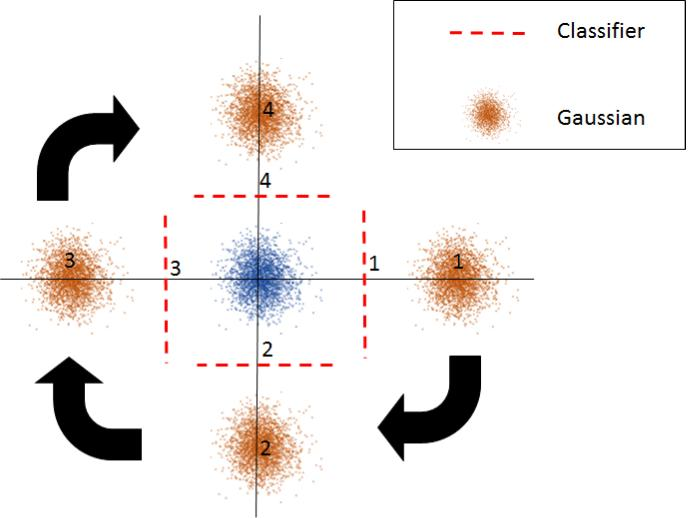
\includegraphics[width=9cm, height=7cm]{graphics/LDA/DataShiftInEarlyDetection.jpg}
	\caption{Illustration of the generation process of the synthetic data.
	The class $P$ (denoted in blue) is fixed, while $Q$ changes three
	times, every 1,500 rounds (the changes are depicted by the dark arrows).
	\ref{PERvsDLDAoverTime}.}
	\label{DataShiftInEarlyDetection}
\end{figure}

Figure \ref{PERvsDLDAoverTime} shows the behavior of the DLDA monitoring
algorithm over the synthetic dataset, with three points in time at which the data abruptly changes. 
DLDA achieves a communication overhead of 0.01 messages per node per round, with the model error guaranteed to always be below the given threshold.
Conversely, the equivalent PER(100) algorithm doesn't maintain the
model error below the threshold (red dashed line).
Figure \ref{PERvsDLDAoverTime} shows that the periodic algorithm does not always 
synchronize when the model drift exceeds a given threshold. 
Moreover, it triggers redundant synchronizations when there is no change in the data.
\begin{figure*}[ht]
	\centering
	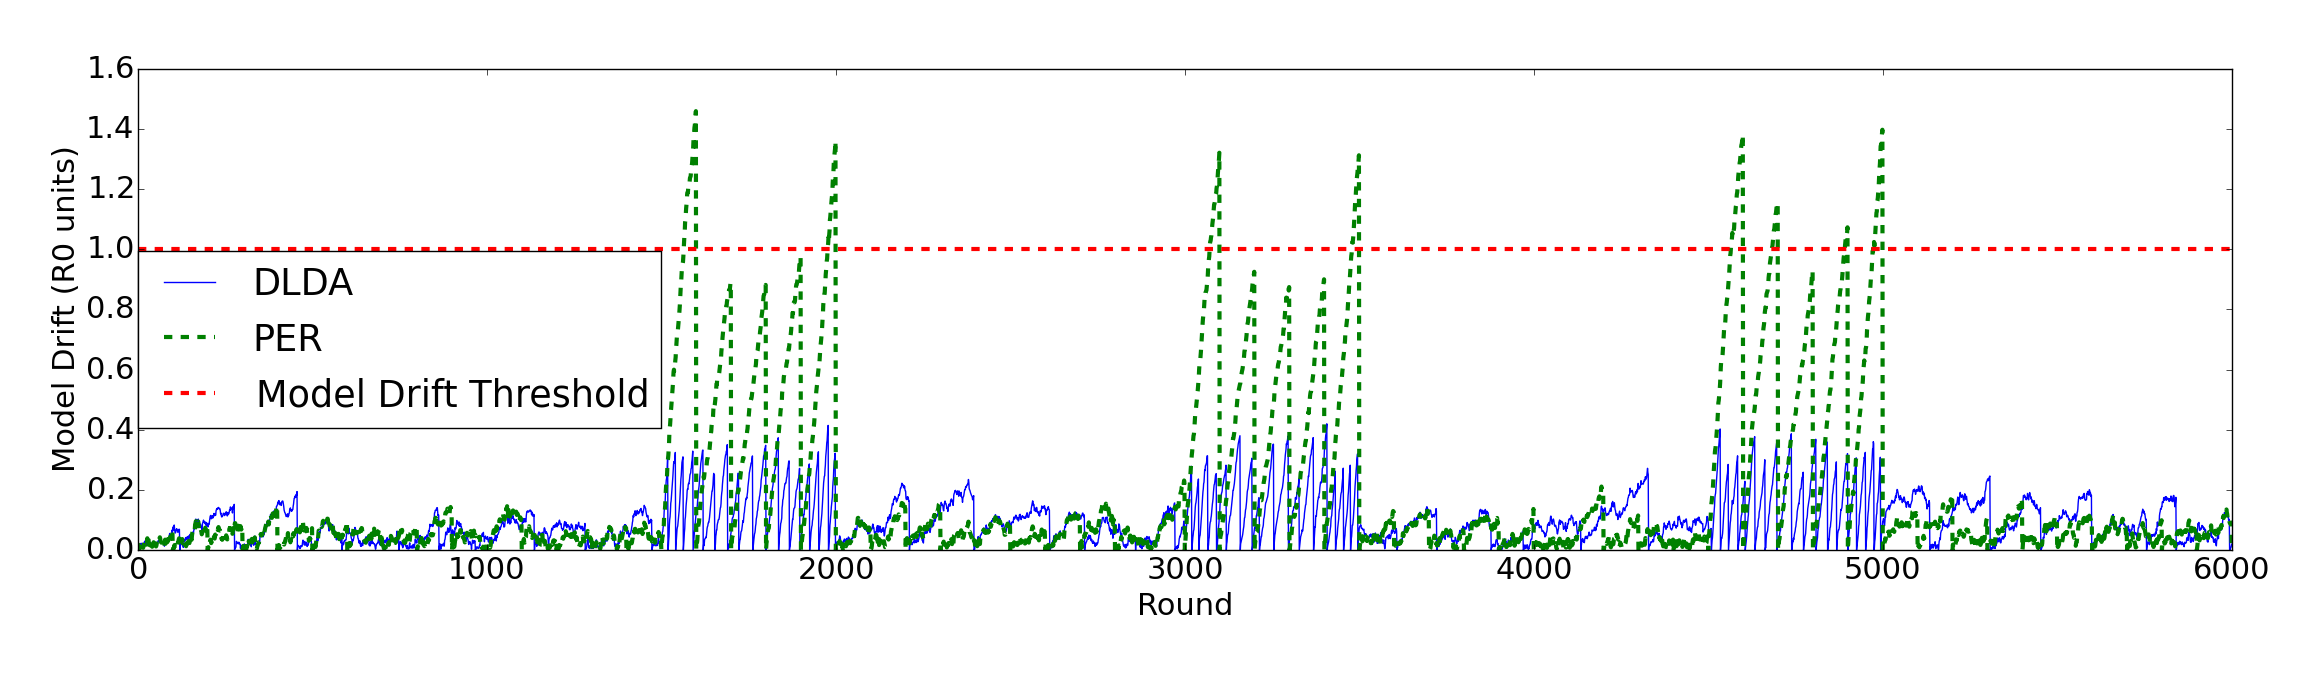
\includegraphics[width=\textwidth, height=7cm]{graphics/LDA/PERvsDLDAoverTime.png}
	\caption{DLDA error (blue) vs. PER(100) error (red), for the synthetic
	data described above. Horizontal axis represents rounds, vertical
	axis represents the norm of the difference between the real (global) model and the current model held at the nodes. Window size is 1,000.
	The maximum allowed error (which DLDA guarantees will never be
	surpassed) is $T = 0.997$ (which corresponds to a difference of
	0.077 radians, or 4.4 degrees, in the classifier's direction). Both
	algorithms transmit the same overall number of bytes, but at different
	rounds; while PER sends alerts periodically, DLDA alerts only when the classifier may have changed. For this reason, PER yields a larger
	error when the two classes (and the classifier) change.
}
	\label{PERvsDLDAoverTime}
\end{figure*}
%
%
\subsubsection{Early Drift Detection}\label{sec:earlydetection}
%
%
To further expound on the advantage of the proposed DLDA algorithm, we consider a toy example (Fig. \ref{EarlyDetection}), 
in which 2D data arrives from two classes ($P$'s samples are shown as plus signs and $Q$'s samples as minus signs). The means of the classes change 
according to the depicted grey arrows, from time $t_1$ to $t_L$. The dark
line at an angle of $-45^{\circ}$ represents the optimal projection
direction at time $t_1$. As the classes change, this initial projection
direction remains "correct", in the sense that it still separates the
two classes; alas, at time $t_L$, the two classes have switched their
positions relative to the projection's direction, and the classifier
fails. Hence, a monitoring algorithm which only checks for misclassification
at the nodes will fail to detect the drift in the classes until it is too
late -- i.e., that the classifier fails -- while DLDA will alert earlier, 
when the real (global) classifier will have changed by more than the
provided threshold (in this case 0.52 radians, or $30^{\circ}$); this point is marked by an arrow in Fig. \ref{EarlyDetection}.
%
\begin{figure}[ht]
	\centering
	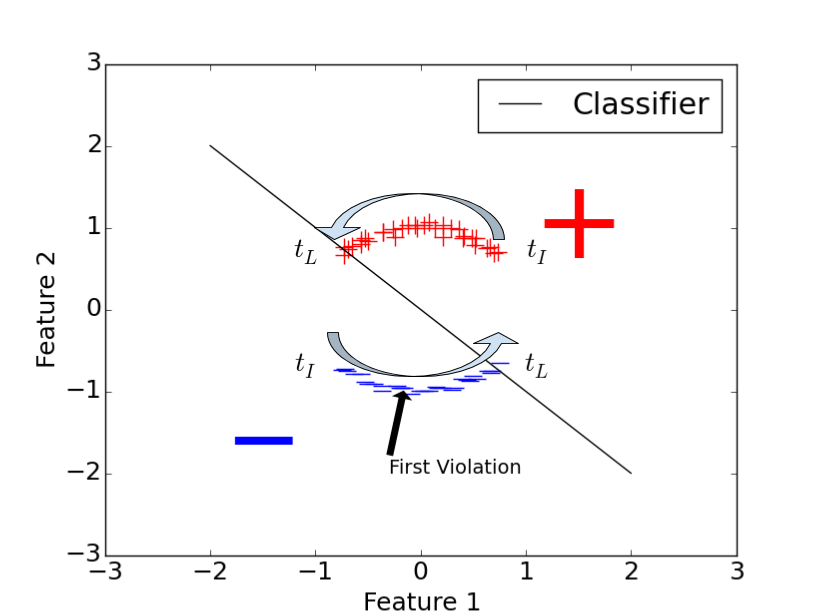
\includegraphics[width=90mm, height=7cm]{graphics/LDA/EarlyDetection.png}
	\caption{A toy example demonstrating early detection of a change in the data.}
	\label{EarlyDetection}
\end{figure}
%
%
\subsubsection{Parameter Analysis}\label{sec:paramanal}
Next, we analyze the parameters of the DLDA algorithm.

\noindent\textbf{Model Drift Threshold:} Model Drift Threshold is given by the user. Above it the model drift is too big. It can be quantified in two ways: as the maximal angle between $w$ and $w_0$, or as the euclidean distance between them. 
Figure \ref{PERvsDLDAoverError} shows the communication requirements of the DLDA algorithm as a function of the model drift threshold, and the minimal communication required to match DLDA using PER.	
It can been seen that for both fixed and dynamic data, DLDA outperforms PER for
any given model drift threshold.
 \begin{figure*}
	\centering
	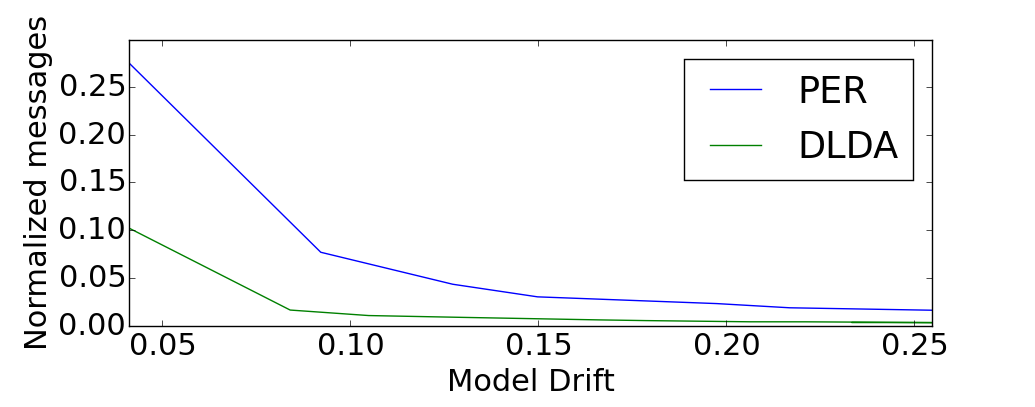
\includegraphics[width=110mm, height=5cm]{graphics/LDA/onlyDrift.png}
	\caption{Communication as the function of model drift for DLDA and PER. The
	periodic algorithm is tuned to achieve the same max model drift as DLDA
	for each model drift threshold.}
	\label{PERvsDLDAoverError}
\end{figure*}

	
\noindent\textbf{Node Scalability:}
Node Scalability is how DLDA performs with different number of nodes.
Figure \ref{Nodes} shows the communication volume as a function of the number of nodes $k$.
We observe that communication increases slowly, reaching 0.25\% on the fixed
data and 0.6\% on the dynamic data distributed across 25 nodes.

\begin{figure}[]
\centering
    \centering
  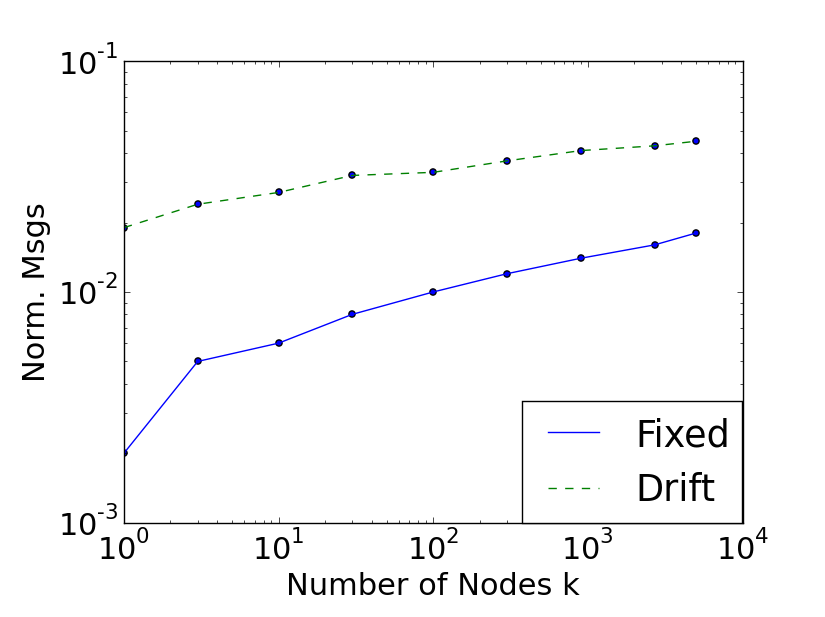
\includegraphics[width=90mm]{graphics/LDA/Nodes.png}
  \caption{Communication as a function of the number of nodes for fixed (blue)
  and changing (green dashed line) datasets}\label{Nodes}
  \end{figure}
 \begin{figure}[]
\centering
  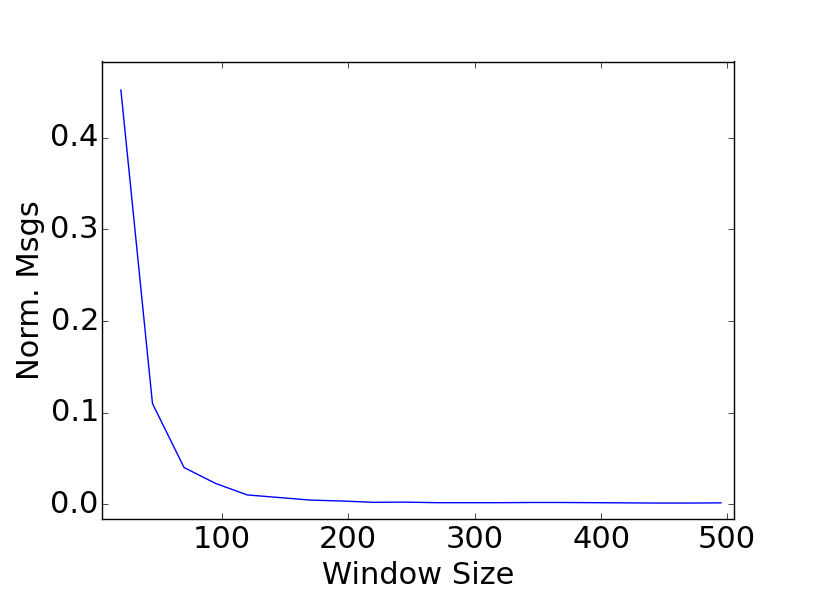
\includegraphics[width=90mm]{graphics/LDA/WindowSize.png}
  \caption{Communication as function of window size }\label{WindowSize}
  \end{figure}
  
  \begin{figure}[]
\centering
  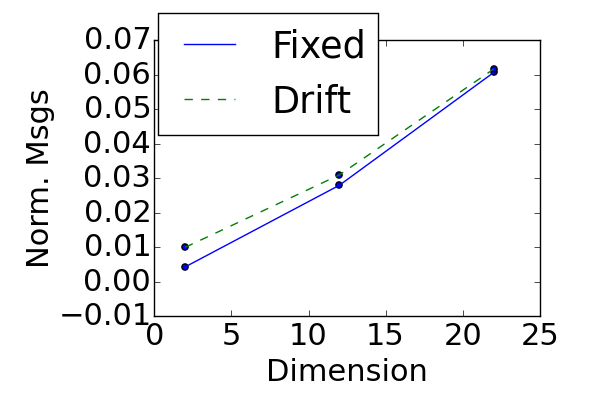
\includegraphics[width=90mm]{graphics/LDA/Dimension.png}
  \caption{Communication as a function of input dimension for fixed (blue) and
  changing (green  dashed line) datasets}\label{Dimension}
\end{figure}

\noindent\textbf{Window Size:}
Figure \ref{WindowSize} shows how communication decreases as a result
of enlarging the window size $W$.  One can increase the window size to compensate for other factors in the system that increase the communication. One of those is
noise (which is quantified in our context by the standard deviation of the
data generating distribution).

%\subsubsection{Noise}
%Figure \ref{Noise} shows normalized messages obtained for different
%noise magnitudes. The experiment shows that the drift grows with the noise, causing more %synchronizations (more communication). This result is not surprising, and the solution is to increase the window size.

Another parameter directly related to the window size is the dimension of the data. The number of samples required for accurate estimation of the covariance matrix grows with the dimension. In our settings, the number of training samples is linked to the window size. When window size is fixed, communication grows linearly with the dimension (see Figure \ref{Dimension}).



\begin{figure}
	\centering
	\includegraphics[width=3.5in,height=2in]{graphics/LDA/DriftDetected.png}
	%\includegraphics[width=\textwidth]{Usenet/DriftDetected.png}
	\caption{Comparison between maximal (over nodes) DLDA model drift (blue)
	and the true global model drift (green dashed line) for $k=2$, $W=450$.
	It can be seen that DLDA responds to the change in the data that occurs
	after 600 rounds (red dotted vertical line) and causes a synchronization in round 698 (blue dashed vertical line).}
	\label{usenet}
	\end{figure}
\subsection{Real Data Experiments}
In this section we test the algorithm on three real data sets. The first
(USENET) is too small to test the probabilistic approach; thus we use this set only for the DLDA test.
The second (Power Consumption Monitoring) is a medium size dataset (it
is distributed over 36 nodes) and we test both DLDA and PDLDA on it.
The third (Gas Sensor Time Series Monitoring) is a big set(it is distributed over
100 nodes). The DLDA synchronization policy is too strict for a large number of nodes; hence we use this set only for the PDLDA test.

\subsubsection{Message Preference Monitoring --- Usenet}
The USENET dataset (~\ref{usenet}) is a text dataset that simulates a stream of messages 
from three newsgroups (medicine, space, baseball); 
the messages are presented sequentially to a user, who then labels them as interesting or junk, 
according to personal interest. 
Attribute values are binary, indicating the presence or absence of the 128 informative words. 
The change in the data occurs from a change in the user's preference (from space to baseball). 
Figure \ref{usenet} shows the results of the DLDA algorithm with $W=450$ . The first 450 rounds over the data correspond to
the initialization phase and are omitted. During the next 50 rounds the DLDA model drift 
(the value is calculated using the left side of the inequality in Eq. \ref{eq:convexBound}) 
increases due to noise in the data; there is no change in the user's
preferences.
From round 500 to 600 the DLDA model drift is stable, and again is due only to the noise. In round 600 there is a concept
drift.
From this point both the DLDA model drift and the true model drift increase until the synchronization in round 698.
\subsubsection{Power Consumption Monitoring}
The Power Consumption dataset contains the hourly power supply of an
Italian electric company as recorded from two sources: power supplied
by the main grid and power transformed from other grids.
This stream contains three-year power supply records
from 1995 to 1998, and our learning task is to predict which hour (1 out of 24 hours) 
the current power supply belongs to. 
Thchange in the dataft in this stream is mainly caused by such factors as season, weather, time of day,
and the differences between working days and weekend.
We demonstrate the algorithms on the following binary classification problem:
given a power supply measurement, decide whether it corresponds to night or day.
This dataset is an example of gradual change in the data (seasons do not
change abruptly).
Figure \ref{PowerSupplyFigures} depicts the results of the DLDA
and PDLDA algorithms. For a small number of nodes, $k=4$, and for large
window size, $W=5000$, DLDA requires only 0.003 normalized messages.
For a more distributed system, $k=36$, and a smaller window
size, $W=600$, DLDA requires 0.09 normalized messages. For PDLDA with
$k=36$ and $W=600$ and a violation threshold (VT) of 50\%, PDLDA
requires 0.02 normalized messages, much better than DLDA in the same setting.

\begin{figure*}
    \centering
    \begin{subfigure}[b]{0.8\textwidth}
        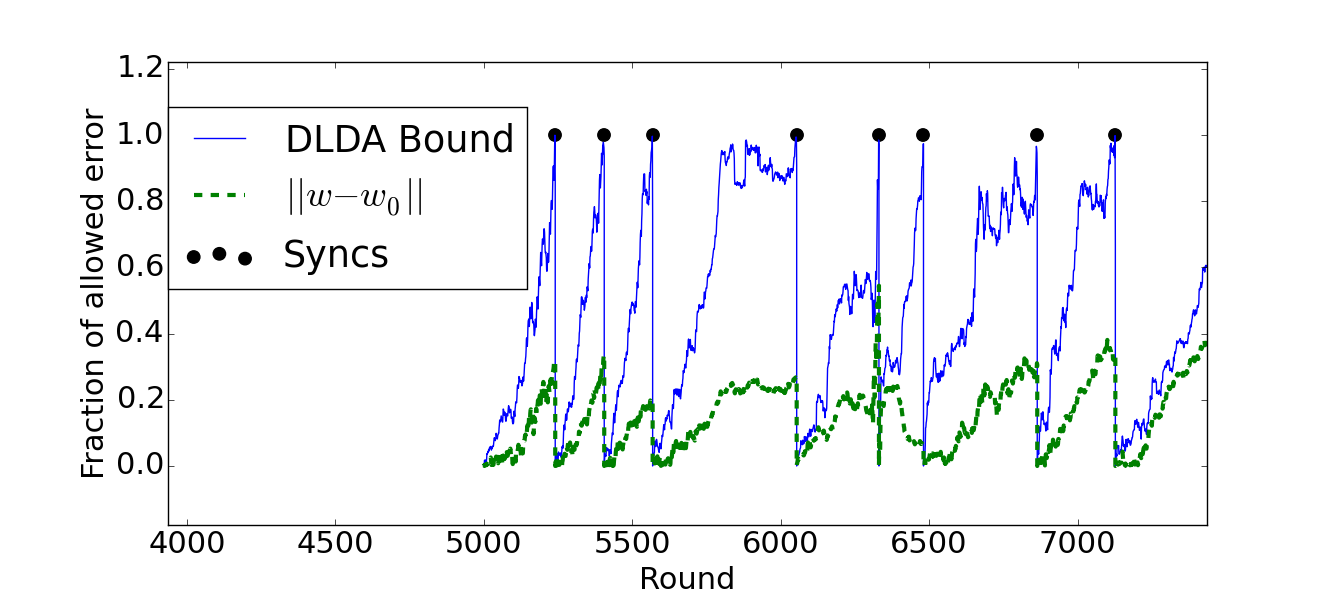
\includegraphics[width=\textwidth]{graphics/LDA/4nodes.png}
        \caption{DLDA behavior on Power Consumption data with: k=4, W=5000, VT=0}
    \end{subfigure}

    \begin{subfigure}[b]{0.8\textwidth}
        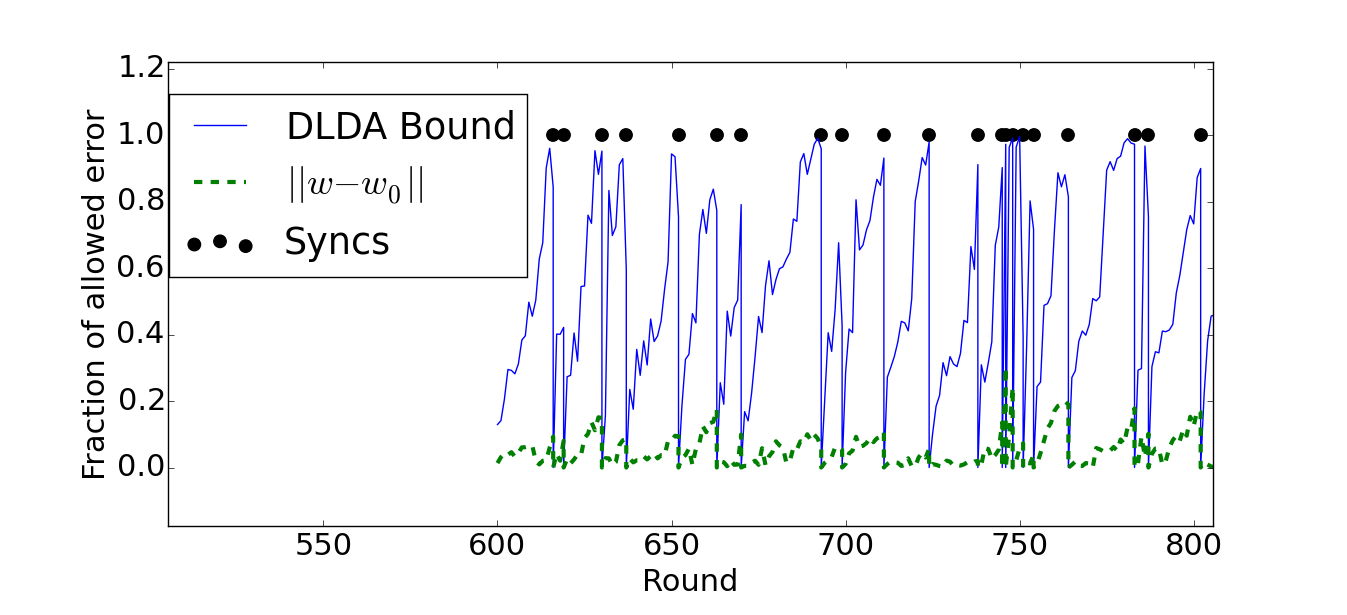
\includegraphics[width=\textwidth]{graphics/LDA/36nodes.png}
        \caption{DLDA behavior on Power Consumption data with: k=36 Nodes, W=600, VT=0}
    \end{subfigure}

    \begin{subfigure}[b]{0.8\textwidth}
        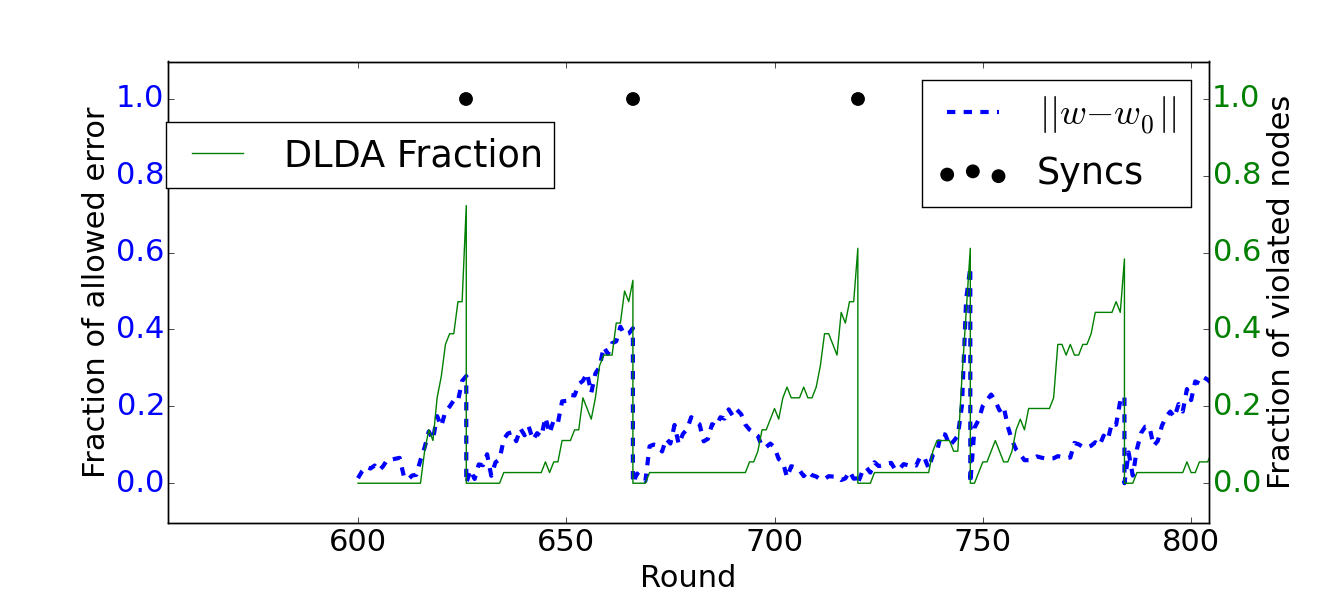
\includegraphics[width=\textwidth]{graphics/LDA/36nodesProb.png}
        \caption{PDLDA behavior on Power Consumption data with: k=36 Nodes, W=600, VT=18}
    \end{subfigure}
    \caption{The top and the center figures show the DLDA algorithm on the Power Supply data set for a small (top) and large (center) number of nodes. The blue line represents the value of the local bound expression, corresponding to the node with the maximum value. The green dashed line shows the model drift (normalized by the threshold); the model is computed after the data was aggregated from all nodes. The bottom plot shows the results of the PDLDA on the same dataset. The blue line in the bottom plot represents the fraction of violated nodes.}\label{PowerSupplyFigures}
\end{figure*}

\subsubsection{Gas Sensor Time Series Monitoring}
\begin{figure*}
\centering
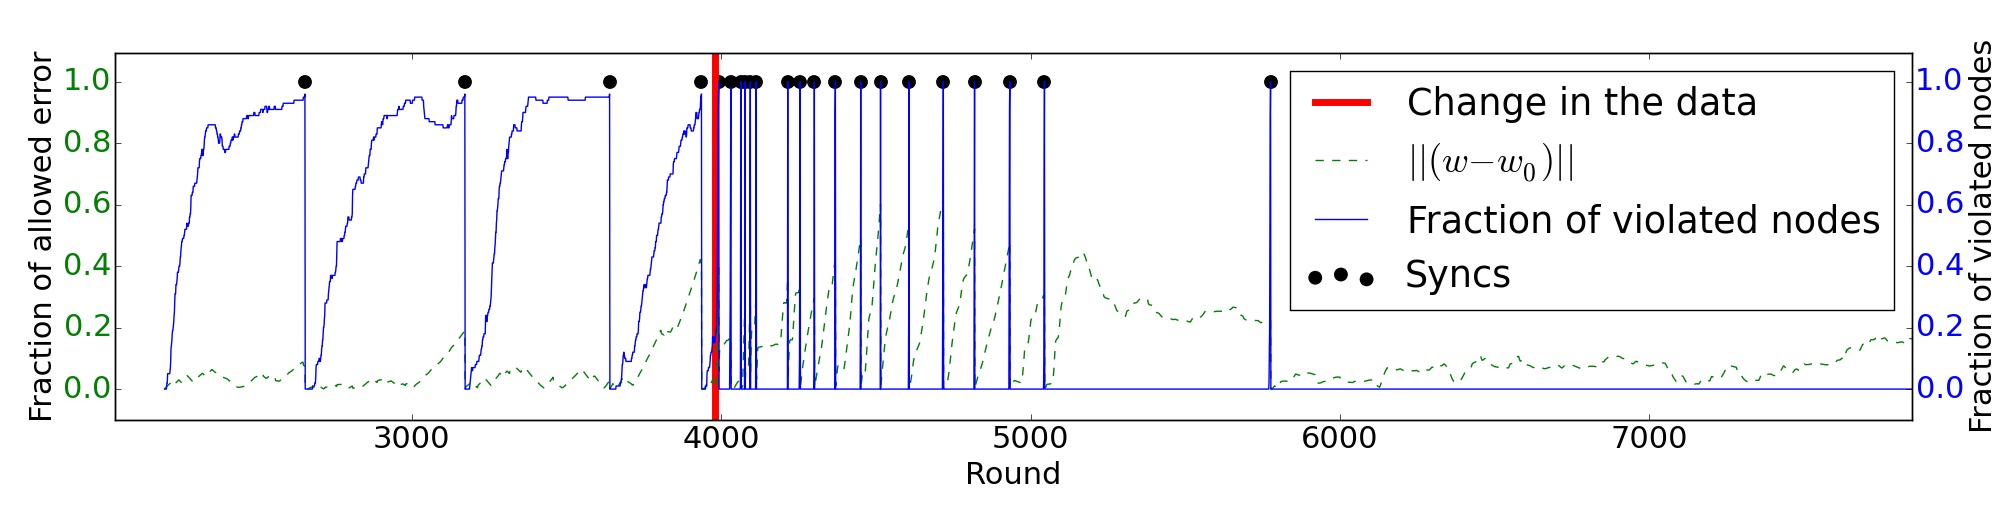
\includegraphics[width=\textwidth]{graphics/LDA/overTime100k.png}
\caption{Demonstration of PDLDA on the Gas Sensor dataset.
A comparison between the true model drift (green) to the fraction of the nodes that
are violated in the current round (blue).
The experiment is configured for k=100 nodes, and the violation threshold is
VT=80.}
\label{BigGasOverTime}
\end{figure*}
Data in this experiment consists of measurements collected
by an array of 16 chemical sensors in a lab, recording at a sampling
rate of 100Hz for 24 hours, resulting in 8378504 data points for each sensor.
During the first 12 hours the task is to detect the presence of carbon monoxide
(CO) in a mixture of chemicals, and from the 13th hour the task is to detect the presence of methane, 
which corresponds to an abrupt change in the data.
Figure \ref{BigGasOverTime} demonstrates the results of PDLDA algorithm.
First, we can observe that the fraction of violated nodes (shown in blue) correlates with the true model drift (shown in green). Second, we can see two patterns of behavior, which are separated by an abrupt switch in the data  (marked by the vertical red line). Before the switch,  the synchronization occurs every 150 rounds, and after the switch, it goes down to every 50 rounds. There is a transition period of about 1000 rounds that follows the point of the data switch. In this interval, the sliding window mixes the old (before switch) data and the new (after the switch) data, but once the window aggregates enough data, the algorithms stabilizes and reduces the communication requirements.   This experiment shows that the PDLDA algorithm detects the abrupt change in the data and adapts to the new conditions after a short period of time.







\thesisbibfiles{bib}
\thesisbibstyle{alpha}





% end of file template.tex



\chapter{Conclusion}
\label{chap:conclusion}
In the first chapter we succeeded with a relatively high success rate to
capture the essence, and develop automatic recognition of 18 LMA motor elements,
using an inexpensive and widely available sensor. We hope that our work will
provide the foundation and inspiration for developing an in-home, inexpensive
LMA based feedback system that will be used for multiple purposes, such as
therapy, arts, video games, communication and human-robot interaction.

In the second chapter we introduced the first communication-efficient monitoring algorithm for a linear classifier model that monitors the
models itself, but does not require knowledge of the global model at the local nodes.
As long as all nodes meet their local condition, the
global model is guaranteed to be valid. Our algorithm has important benefits:
\begin{itemize}
  \item Our method works with distributed data in a communication efficient way.
  \item Monitoring the model as opposed to monitoring the misclassifications
  allows for early detection of the changing even before misclassification
  occurs.
\end{itemize}

We evaluated the theoretical scheme -- DLDA, and its probabilistic version -- PDLDA, on three real data sets.
For a small number of nodes we used DLDA with its theoretical guarantee, and for a greater number of nodes we used
PDLDA. We showed that the proposed scheme outperforms PER: it maintains a smaller Euclidean distance between
the last computed model and the current true model with a lower volume of communication.
This work is the first step in designing communication-efficient algorithms
with theoretical guarantees for monitoring classification models over dynamic distributed data streams. One of the future directions is to extend the proposed framework to
ensembles of linear classifiers and neural networks, including deep learning networks.




%
% Add any appendices here; they must come _before_ the bibliography
%


%\appendix
%\noappendicestocpagenum
%\addappheadtotoc



%\chapter{Appendix}
\label{appendix:Appendix}

\section{Appendix 1: proof of the convex bound in Lemma 2}
\label{sec:appendix1}
We must find a convex subset $\mathcal{C}$ satisfying the condition of Eq. \ref{convex}. Let
us start by recalling the definition of the operator norm of a matrix:
\begin{definition}
Let $A$ be a matrix. Its operator norm or
spectral norm (hereafter just norm), is defined as:
\begin{equation}
\Big \| A \Big \| = \sup_{x \neq 0}\frac{||Ax||}{||x||}.
\end{equation}
\end{definition}
The following result is very useful in the forthcoming analysis:
\begin{lemma} \label{lemma:newman}
If $A$ is square and $\Big \| A \Big \| < 1$, then
\begin{equation*}
\Big \| (I+A)^{-1} \Big \| < \frac{1}{1- \Big \|A \Big \|}.
\end{equation*}
\end{lemma}
The proof for this lemma can be found in \cite{gabel2015monitoring}.

\subsection{Convex Bound Proof}
We recall that $\mathcal{C}$ is the convex subset that satisfies
inequality \ref{convex}, and $\mathcal{G}$ is the set of triplets
$(\Delta_s^i, \delta_p^i, \delta_q^i)$
which satisfy the inequality \ref{eq:convexBound}.

\begin{lemma} \label{GinC}
%$\mathcal{G} \subseteq \mathcal{C}$:
\begin{equation}
\begin{split}
(||B_0^{-1}\delta|| + (||w_0||+R_0)(\Big \|B_0^{-1}L\Big \|+\Big \|B_0^{-1}M\Big \|) \\
 \leq R_0) \Rightarrow (||w-w_0|| \leq R_0).
\end{split}
\end{equation}
\end{lemma}

\begin{proof}
We can write the sphere inclusion condition \ref{eq:critiria} in terms of $B_0, \Delta, u_0$ and $\delta$, by using the triangle inequality:
\begin{equation} \label{in}
\begin{split}
||w-w_0|| & = \ ||(B_0+\Delta)^{-1}(u_0+\delta) - B_0^{-1}u_0|| \\
& < ||(B_0+\Delta)^{-1}\delta|| \\
& \ \ + ||((B_0+\Delta)^{-1} - B_0^{-1})u_0||.
\end{split}
\end{equation}

We split the right side of the last inequality into two parts:
\begin{equation}  \label{e1e2}
\begin{split}
& E_1:= ||(B_0+\Delta)^{-1}\delta|| \\
& E_2:= ||((B_0+\Delta)^{-1} - B_0^{-1})u_0||.
\end{split}
\end{equation}
Under the assumption  $||B_0^{-1}\Delta||\ \leq \ 1$,
it follows from lemma \ref{lemma:newman}:
\begin{equation} \label{e1e2In}
\begin{split}
& E_1 \leq \frac{||B_0^{-1}\delta||}{1-\Big \|B_0^{-1}\Delta\Big \|} \\
& E_2 \leq  \frac{|| B_0^{-1}\Delta w_0||}{1-\Big \|B_0^{-1}\Delta\Big \|}.
\end{split}
\end{equation}
From standard properties of the norm we get:
\begin{equation} \label{CS}
||B_0^{-1}\Delta w_0||  \leq  \Big \|B_0^{-1}\Delta \Big \| ||w_0||.
\end{equation}
Substituting Eq. \ref{e1e2}, \ref{e1e2In} and \ref{CS} in Eq. \ref{in}, we
get:
\begin{equation}
\begin{split}
|| w-w_0 \parallel & \leq \ E_1+E_2 \\
& \leq \frac{||B_0^{-1}\delta|| + \Big \|B_0^{-1}\Delta\Big \|||w_0||}{1 -\Big \|B_0^{-1}\Delta \Big \|} \\
& \leq R_0.
\end{split}
\end{equation}
After rearranging the terms, we have
\begin{equation} \label{lostDenom}
||B_0^{-1}\delta|| + \Big \|B_0^{-1}\Delta \Big \| ||w_0||
\leq R_0(1 -\Big \|B_0^{-1}\Delta\Big \|).
\end{equation}
From the triangle inequality we can rewrite:
\begin{equation} \label{linQuad}
\Big \|B_0^{-1}\Delta\Big \| \leq \Big \|B_0^{-1}L\Big \|+\Big \|B_0^{-1}M\Big \|.
\end{equation}
And finally, combining inequalities \ref{lostDenom} and \ref{linQuad},
we get the following bound:
\begin{alignat*}{2} \label{convexBound}
&||B_0^{-1}\delta|| &+ (||w_0||+R_0)(\Big \|B_0^{-1}L\Big \|+\Big \|B_0^{-1}M\Big \|)  \leq R_0. \\
&
\end{alignat*}
\end{proof}

\begin{lemma} \label{GisConvex}
$||B_0^{-1}\delta|| + (||w_0||+R_0)(\Big \|B_0^{-1}L\Big \|+\Big \|B_0^{-1}M\Big \|$ is convex in $(\Delta_s,\delta_p, \delta_q).$
%$||B_0^{-1}\delta||$ is convex in $\delta$.
\end{lemma}
\begin{proof}
Multiplication by $B_0^{-1}$ is a linear operation, and norm is a convex
operation. Therefore $||B_0^{-1}\delta||$ is convex in $\delta$.
%\end{proof}

We recall that:
\begin{equation*}
L:= \Delta_S - p_0\delta_p^T - \delta_pp_0^T - q_0\delta_q^T - \delta_qq_0^T.
\end{equation*}
%\begin{lemma} \label{L}
%$||B_0^{-1}L||$ is convex in $\Delta_s, \delta_p$
%and $\delta_q$.
%\end{lemma}
%\begin{proof}
$L$ is linear in $(\Delta_s, \delta_p)$ and therefore $\Big \|B_0^{-1}L\Big \|$ is convex in these variables.

%\end{proof}

We recall that:
\begin{equation*}
M:= - \delta_p\delta_p^T - \delta_q\delta_q^T.
\end{equation*}

%\begin{lemma} \label{M}
It is left to prove that $\Big \|B_0^{-1}M\Big \|$ is convex in $(\delta_p, \delta_q)$.
%\end{lemma}
%\begin{proof}
\\From the definition of the operator norm, we can rewrite:
\begin{alignat*} {2}
\Big \|M \Big \| & = && ||B_0^{-1}(\max_{||u||=1}{\{u^T \delta_p\delta_p^T u\}} +
\max_{||u||=1}{\{u^T \delta_q\delta_q^T u\}})||\\
& = && ||B_0^{-1}(\max_{||u||=1}{\{||u^T \delta_p||^2\}} +
\max_{||u||=1}{\{||u^T \delta_q||^2\}})||.
\end{alignat*}
\\We observe that the maximum over any number (infinite in this case) of convex functions
 is also a convex
function, and since multiplication by a matrix and the norm
operation preserve convexity, this concludes the proof.
\end{proof}

\begin{corollary}
From Lemmas \ref{GinC} and \ref{averages}, we conclude that $\mathcal{G}\subseteq \mathcal{C}$. From Lemma \ref{GisConvex} we conclude that $\mathcal{G}$ is convex, and this completes the proof of Lemma \ref{lemma:convexBound}.
\end{corollary}
%
%
\section{Appendix 2: an analysis of the probabilistic version, PDLDA}
%
\label{sec:prob}
As briefly discussed in Section \ref{sec:PDLDA}, the DLDA synchronization policy
(a node alerts whenever its local vector exits the convex set $\mathcal{C}$) is
strictly correct (i.e. every global violation will be caught; recall that a global
violation occurs when the average vector exits $\mathcal{C}$). However, typically,
even if a relatively large percentage of the local vectors are not in 
$\mathcal{C}$, the average is still in $\mathcal{C}$, due to a "cancellation effect"
which resembles the one manifest in the central limit theorem. While the
treatment of general convex sets is difficult and left for future work,
we discuss here the case in which $\mathcal{C}$ is a solid sphere; this can
be directly applied to spherical safe zones, which have proven to be simple and
effective \cite{keren2012shape}. 

Assume then the following: given are $k$ nodes, with node $i$ 
holding a vector $v_i$. If the safe zone is
a solid sphere of radius $R$, assumed without loss of generality to
be centered at the origin, the monitored global condition is 
$\norm{\left(\displaystyle \sum_{i=1}^k v_i\right)/k} \leq R$, while
a  node $i$ violates if $||v_i|| \leq R$. In order to continue the analysis,
we must define some probabilistic model over $v_i$; we assume that the
$v_i$ are independent Gaussian vectors, with zero mean and a covariance
matrix equal to $\sigma I$ ($I$ is the $n \times n$ unit matrix, where
$n$ is the dimension of the $v_i$'s). The
following analysis, especially the "cancellation effect" when averaging
the $v_i$'s, will hold for other distributions as well; we use the Gaussian
one since it is the most common.

Recall that all the local drift vectors are initially (i.e. after a 
full synchronization) 
equal to zero; hence, the local vectors $v_i$ are initially all zero, and 
gradually their magnitude increases. We therefore assume that $\sigma$
increases with time, and with it the magnitude of $||v_i||$. We next
compute, for a given $\sigma$, the expectation and variance of both 
$||v_i||^2$ and $\norm{\left(\displaystyle \sum_{i=1}^k v_i\right)/k}^2$,
which will allow to estimate the probabilities of them crossing $R^2$
(which is equivalent to local vs. global violation).
%
%
\subsection{The distribution of the norm squared at a single node}
\label{sec:vi2}%
%
In order to reduce equation clutter, we will assume that $\sigma=1$ (the
general case follows immediately by scaling). The probability density 
of every coordinate $x$ of $v_i$ (for all $i$) is that of the standard
normal distribution, $\frac{1}{\sqrt{2\pi}}\exp{(-x^2/2)}$. The expectation
of the square of every coordinate is of course just 1, hence the 
expectation of the norm squared is the dimension $n$.

To compute the variance of $||v_i||^2$, we need to first compute the
expectation of its square, that is, $||v_i||^4$. Representing $v_i$'s
coordinates by $x_1 \ldots x_n$, this requires
computing the integral
\begin{eqnarray*}
& & \frac{1}{{(2\pi)}^{n/2}}\displaystyle\limits\int_{-\infty}^{\infty} \ldots \limits\int_{-\infty}^{\infty}(x^2_1 + \ldots x^2_n)^2 \exp{(-1/2)(x^2_1 + \ldots x^2_n)) \\
& & dx_1 \ldots dx_n
\end{eqnarray*}
expanding the square yields both fourth powers $x_i^4$ and products of the form
$x_i^2x_j^2$. Due to symmetry considerations, all corresponding integrals of the first
type are equal, and similarly for the second. This rather straightforward leads
to the result being equal to $n^2+2n$. The variance therefore equals 
$(n^2+2n)-n^2=2n$.
%
%
\subsection{The distribution of the norm squared of the average vector}
%
%
This distribution is somewhat more complicated. We leave out the $k^2$ constant
for the meanwhile (it will be factored in when the computation is done). Note
that
\begin{equation}
\label{proof-2-1}
\norm {\displaystyle \sum_{i=1}^k v_i}^2 = 
\displaystyle \sum_{i=1}^k \norm{v_i}^2 +
\displaystyle \sum_{i \neq j}^k } \langle v_i , v_j\rangle
\end{equation}
%

The first summand is just the sum of norms squared, and it was treated in
Section \ref{sec:vi2}. We turn to the second summand. Due to symmetry considerations,
it suffices to compute the distribution of $\langle v_i , v_j\rangle$ for
any choice of $i \neq j$, so we assume that $x,y$ are vectors drawn from the
same distribution as the $v_i$'s (multivariate standard normal), and study
the distribution of $\langle x,y\rangle$. Since 
$\langle x,y\rangle = \displaystyle\sum_{i=1}^n x_iy_i$, and since all
$x_i,y_i$ are zero mean and independent, the expectation of 
$\langle x,y\rangle$ is also zero. To compute the variance, we need
to evaluate the integral of $\langle x,y\rangle^2$; this standard Gaussian
integral turns out to equal $n$. 

Combining the results on the expectation and variance of the two summands
($\sum_{i=1}^k \norm{v_i}^2$ and $\sum_{i \neq j}^k \langle v_i , v_j\rangle$),
using independence and then dividing by $k^2$, yields the following (for a 
general $\sigma$):

\begin{lemma}
\label{lemma:Gaussian}
The expectation of the random variable $||v_i||^2$ is $n\sigma^2$, and its
variance is $2n\sigma^4$. Recall that this random variable represents the
data in a single node, and when it crosses $T^2$, a local violation occurs. 


The expectation of the random variable
\(\norm{\left(\displaystyle \sum_{i=1}^k v_i\right)/k}^2\) is
$\frac{n\sigma^2}{k}$, and its variance is 
$\frac{2n\sigma^4}{k^3} + \frac{n\sigma^4}{k^2} \approx \frac{n\sigma^4}{k^2}$.
Recall that this random variable represents the
global data, and when it crosses $T^2$, a global (i.e. {\emph real}) violation occurs. 
\end{lemma}

To summarize, the (not too surprising) result is that both the expectation and
standard deviation of the global vector's norm squared are smaller by a factor of $k$ than those of the local vector's norm squared. Note that the distribution of the norm
squared of the local vectors is strongly peaked (i.e. the standard deviation,
$\sqrt{2n}\sigma^2$, is much smaller than the expectation, $n\sigma^2$). This means
that, with a very good approximation, the local nodes start reporting violations
when $n\sigma^2=T^2$, or $\sigma = T/\sqrt{n}$. But for this $\sigma$, the 
expectation and standard deviation of the norm of the global vector squared
are equal to $T^2/k$ and $T^2/k\sqrt{n}$. Since, from the central limit theorem,
the distribution approximates a normal one, it is clear that -- since both its
expectation and standard deviation are smaller than $T^2$ by a factor of at least
$k$, then the probability that this variable crosses $T^2$ is extremely small (and
it decreases when the number of nodes increases).

Note that, in the above analysis for computing the expectation and variance
of the norm squared of the local and global vectors, we did not strongly rely
on the properties of the assumed normal distribution. Indeed, the same type
of analysis could have been carried out by merely assuming any values of
expectation and variance for the local vectors, and the results would be
similar in nature, due to the "cancellation effect" manifest in averaging
random variables. The additional factor that can affect the results is the
level of independence between the vectors in different nodes. For fully
independent vectors, the results will be as in the analysis above; in the
adversarial scenario -- all local vectors are equal -- the average vector is just
equal to the local ones, but then, the probabilistic version (PDLDA) will
still be correct. The cases in-between -- i.e some degree of correlation
among the nodes, 
measure by the angles between the local vectors, -- can still be analyzed
as above, and the percentage of nodes that must alert can be tuned to
the strength of this correlation. Space limitation do not allow us to 
pursue this analysis here.





% Back Matter
% ------------

% The following command will typeset the bibliography,
% then typeset the Hebrew part of the thesis:
% - Cover page
% - Title page
% - Acknowledgements page
%  (NO table of contents or list of figures in Hebrew)
% - (Extended) abstract (1000-2000 words)
%
% based on information you've provided in the thesis-fields file
% (including the relative paths to your bib files). The Hebrew
% content will be typeset in _reverse_page_order_, i.e. first
% in the file will be the last page of the abstract, and the
% Hebrew cover page will be the last page of the file.
%
\makebackmatter

% The resulting PDF can be printed and taken straight to binding,
% i.e. you do not need to flip any pages anywhere. Of course,
% mind the LaTeX error and warning messages, overfull hboxes etc.




\end{document}
 